\documentclass[11pt,a4paper]{article}
\usepackage[margin=24mm]{geometry}
\usepackage[T1]{fontenc}
\usepackage{lmodern,microtype,amsmath,amssymb,bm,booktabs,longtable,array,graphicx,xcolor,listings}
\usepackage{enumitem,natbib,tikz,xurl,hyperref}
\usetikzlibrary{arrows.meta,positioning}
\hypersetup{colorlinks=true,linkcolor=blue!45!black,citecolor=blue!45!black,urlcolor=blue!45!black,pdftitle={ESF-IGRF-AMR Methods and Implementation Reference},pdfauthor={ESF-IGRF-AMR contributors}}
\setlength{\emergencystretch}{3em}
\setlist{nosep,topsep=4pt}
\lstset{basicstyle=\ttfamily\footnotesize,breaklines=true,columns=fullflexible,keepspaces=true,frame=single,showstringspaces=false}
\newcommand{\code}[1]{\texttt{\detokenize{#1}}}
\newcommand{\bn}{\bm n}
\newcommand{\bb}{\bm b}
\newcommand{\bE}{\bm E}
\newcommand{\bJ}{\bm J}
\newcommand{\bx}{\bm x}
\newcommand{\bu}{\bm u}
\newcommand{\bg}{\bm g}
\newcommand{\kb}{k_{\rm B}}
\newcommand{\dd}{\mathrm d}
\title{An Inspectable Field-Aligned ESF Solver with IGRF Geometry,\newline Conservative Anisotropic AMR, and Hybrid Parallel Kernels\\[4pt]\large Physics, numerical algorithms, and a function-level implementation reference}
\author{ESF-IGRF-AMR contributors}
\date{Version 0.1.0 methods manuscript and teaching reference}
\begin{document}
\maketitle
\begin{abstract}
We describe an independently implemented C11 electrostatic model for nonlinear
equatorial spread F on complete conjugate magnetic flux tubes. Traced IGRF-14
or dipole geometry is combined with conservative O$^+$ density and parallel
momentum evolution, field-line-integrated Pedersen/Hall current closure, and
two- or three-level refinement transverse to the magnetic field. The adaptive
density approximation is segmented along each tube without refining the
field coordinate. An optional reduced night module transports NO$^+$ and
O$_2^+$, evaluates a four-reaction network, and uses a common quasineutral
electron pressure. We derive the actual discrete fluxes, exponential drag
update, constrained potential assembly, background-preserving transfer and
solution-based refinement/coarsening criteria. Explicit ownership and cache
contracts explain which kernels can be threaded and why others remain
serial within each MPI process. Validation distinguishes algebraic residual,
conservation, saved-field parity, geometry, and physical interpretation.
The implementation remains isothermal with prescribed neutrals and omits
photoionization and several multi-fluid couplings. It is not an exact TELF
port or an observation-calibrated forecast. A complete parameter reference,
function catalog and separate annotated-source atlas make the frozen methods
auditable and suitable for student use.
\end{abstract}
\noindent\textbf{Manuscript status.} This is a software methods manuscript,
not a claim of peer review or publication. Scientific case calibration,
long-time discretization sensitivity and observational validation remain
separate research tasks. Reproduce a result using its exact release tag,
source identity, effective case and input hashes.
\tableofcontents
\clearpage
\section{Purpose and relation to previous ESF models}
The instability problem requires weak numerical diffusion, closure through
the conjugate ionosphere, and a consistent coupling between plasma density
and polarization potential. The two-dimensional study of
\citet{Li2021} and the three-dimensional TELF study of \citet{Li2023} motivate
the scientific problem and the need to retain parallel flow and realistic
integrated conductivity. This code is an independent implementation with
different geometry, potential backend, limiter stencil, parallel relaxation
and adaptive layout. Agreement of qualitative morphology does not establish
an exact reproduction of either paper.

The primary design goal is an inspectable reduced model: the physical
closure, mathematical discretization, implementation and measured validation
are described separately. No TELF, Athena++ or SWMF source is incorporated.
The latter frameworks inform the conservation, hierarchy and parallel-ownership
audit, rather than providing a drop-in ESF solver.

\section{State, units and physical approximations}
Let $n_s$ be SI number density, $u_s$ the signed velocity along the discrete
magnetic tangent $\bb$, and $m_s$ an ion mass. Species are O$^+$, and optionally
NO$^+$ and O$_2^+$, with masses $16,30,32$ atomic mass units. Electron inertia
is neglected. Stored fields are
\begin{equation}
 N_s=n_s/n_*,\qquad M_s=N_su_s,\qquad n_*=10^{12}\ {\rm m}^{-3}.
\end{equation}
Thus $M_s$ is number momentum in normalized density units, not mass density
times velocity. All three ions are singly charged. In the transported night
module,
\begin{equation} n_e=n_{\rm O^+}+n_{\rm NO^+}+n_{\rm O_2^+}.\label{eq:ne}\end{equation}
Without that module a separately prescribed molecular E-region population
provides additional electrons and conductivity; it is not another transported
O$^+$ Chapman component.

The temperatures, neutral densities, geomagnetic field and geometry are
prescribed. There is no energy equation, evolving neutral wind, ion-ion
momentum transfer, full reactive momentum exchange, molecular perpendicular
pressure diffusion or photoionization. Gravity is
\begin{equation}
 \bg=-9.8(a/r)^2\hat{\bm r},\qquad a=6371200\ {\rm m}.
\end{equation}
These omissions constrain physical interpretation even when numerical
conservation and residual tests pass.

\subsection{Continuity and field-aligned momentum}
The transported continuity equation is
\begin{equation}
 \partial_t n_s+\nabla\cdot[n_s(\bu_{\perp s}+u_s\bb)]=S_s.
 \label{eq:continuity}
\end{equation}
The parallel pressure/gravity/neutral-drag acceleration used by the relaxation
branch is
\begin{equation}
 \partial_t M_s=\mathcal T_s+
 N_s\left[g_\parallel-\frac{\kb}{m_s}
 \left(T_i\partial_\parallel\ln n_s+T_e\partial_\parallel\ln n_e\right)\right]
 -\nu_sM_s+\mathcal C_{M_s}.
 \label{eq:momentum}
\end{equation}
$\mathcal T_s$ denotes the conservative advective momentum flux described
below. The pressure term is not duplicated as an independent pressure flux
in this branch. The optional nonrelaxation reference branch instead retains
a Rusanov pressure flux and its variable-area geometric source. The release
night cases explicitly choose relaxation and fixed $T_i+T_e=2500$ K.

O$^+$ perpendicular mass transport uses
\begin{equation}\bu_{\perp\rm O^+}=\bE\times\bb/B,\qquad \bE=-\nabla\Phi.\end{equation}
The polarization forcing retains gravity currents. Consequently this is a
reduced F-region transport approximation, not a full perpendicular O$^+$
force-balance evolution. Molecular perpendicular transport uses the
species-dependent collisional expression
\begin{align}
 \bu_{\perp s}&=h_s\frac{\bE\times\bb}{B}
              +p_s\frac{\bE_\perp}{B}+\bu_{g,s},\\
 h_s&=\frac{\Omega_s^2}{\nu_s^2+\Omega_s^2},\quad
 p_s=\frac{\nu_s\Omega_s}{\nu_s^2+\Omega_s^2},\quad
 \Omega_s=eB/m_s,\\
 \bu_{g,s}&=\frac{\nu_s\bg_\perp-\Omega_s\bb\times\bg_\perp}
                  {\nu_s^2+\Omega_s^2}.
 \label{eq:mobility}
\end{align}
The weak-collision electric term tends to E-cross-B. This transport is
evaluated through physical faces in all coordinate directions, including
faces normal to the nonorthogonal field-coordinate label.

\subsection{Conductivity and electrostatic closure}
For $\kappa_s=|q_s|B/(m_s\nu_s)$, the quasineutral ion-electron pair responses
used in the code are
\begin{align}
 \sigma_{P,s}&=\frac{en_s}{B}
  \left[\frac{\kappa_s}{1+\kappa_s^2}
       +\frac{\kappa_e}{1+\kappa_e^2}\right],\\
 \sigma_{H,s}&=\frac{en_s}{B}
  \left[\frac{1}{1+\kappa_s^2}-\frac{1}{1+\kappa_e^2}\right].
\end{align}
Summing over ion species counts the electron density once through
Equation~\eqref{eq:ne}. The sign convention is
$\bJ_H=\sigma_H\bb\times\bE$. With $\bJ_g$ the charge-weighted difference
of ion and electron gravity drifts,
\begin{equation}
 \bJ_\perp=\sigma_P\bE_\perp+\sigma_H\bb\times\bE_\perp+\bJ_g.
\end{equation}
Equipotential field lines give $\Phi=\Phi(\xi,\eta,t)$ and the weak equation
\begin{equation}
 \int_V \nabla w\cdot[\sigma_P\nabla\Phi+
 \sigma_H\bb\times\nabla\Phi]\,\dd V
 =\int_V\nabla w\cdot\bJ_g\,\dd V+\mathcal B(w).
 \label{eq:weak}
\end{equation}
The volume spans both conjugate ends. Let $\bg^1=\nabla\xi$ and
$\bg^2=\nabla\eta$. Canonical cell contributions are
\begin{align}
 K_{11}&=V\sigma_P\bg^1\cdot\bg^1,&
 K_{22}&=V\sigma_P\bg^2\cdot\bg^2,\\
 K_{12}&=V[\sigma_P\bg^1\cdot\bg^2+
            \sigma_H\bg^1\cdot(\bb\times\bg^2)],&
 K_{21}&=V[\sigma_P\bg^1\cdot\bg^2-
            \sigma_H\bg^1\cdot(\bb\times\bg^2)],\\
 C_\alpha&=V\bJ_g\cdot\bg^\alpha.&&
\end{align}
The two cross terms must not be conflated. Summing the canonical contributions
along the field provides the transverse element data. A depleted F-region
cell alone does not eliminate the integrated E-region conductance. However,
the night model allows its physical molecular population to react and move;
it does not impose an indefinitely fixed minimum conductance.

\subsection{Boundary and imposed-field policies}
Polarization potential is fixed to zero on the two apex-height extremes.
Regional longitude sides impose $\partial_\xi\Phi_{\rm pol}=0$ while retaining
Hall/nonorthogonal current terms in $\mathcal B$. This differs from
$\bJ\cdot\bn=0$. If regional sides are disabled, the corresponding
nonperiodic sides have prescribed potential. Periodicity is a restricted
aligned-dipole verification option.

A prescribed eastward driver is mapped as
\begin{equation}
 \Phi_{\rm ext}=-L_E E_E(t)(\xi-1/2),
\end{equation}
where $L_E$ is the recorded reference east scale. This specifies a label-space
forcing, not a spatially uniform geographic east field throughout an IGRF
domain. A CSV driver is piecewise linear, must cover the full requested time,
and steps land on its knots. Constant and CSV forcing are mutually exclusive.
Particle-open boundaries use extrapolated exterior states; closed field ends
reflect $u_\parallel$ and set particle flux to zero. Signed boundary flux is
accumulated in the conservation ledger.

\section{Geomagnetic field and traced finite-volume geometry}
\subsection{IGRF evaluation and coordinates}
The included official IGRF-14 coefficients define the Schmidt semi-normalized
internal potential \citep{IGRF14,NOAAIGRF}
\begin{equation}
 V_B=a\sum_{\ell=1}^{L}\left(\frac a r\right)^{\ell+1}
 \sum_{m=0}^\ell(g_\ell^m\cos m\lambda+h_\ell^m\sin m\lambda)
 \overline P_\ell^m(\cos\theta),\quad \bm B=-\nabla V_B.
\end{equation}
The evaluator interpolates five-year epochs and uses the supplied secular
variation for 2025--2030; returned ECEF field is in tesla. Degree13 is IGRF,
degree1 retains the actual tilted dipole coefficients, and aligned-dipole
explicitly substitutes an axis-aligned $g_1^0$ fixture. WGS84 geodetic target
positions and the spherical model-altitude reference remain distinct.

At each apex longitude/radius, a root solve finds radial $B=0$ within the
declared low-latitude bracket. RK4 integrates the unit tangent to the two
spherical base boundaries. The resampling coordinate has increment
\begin{equation}
 \dd\zeta=\frac{\dd\ell}{H_g(h)},\qquad
 H_g(h)=\max[8000,\min(80000,8000+0.12(h-h_b))]\ {\rm m}.
\end{equation}
$N_\parallel+1$ points (\code{ns} segments) are uniform in the joined weighted coordinate, not in arc
length. Grid generation rejects escaped traces, degenerate cells and changes
of Jacobian sign; it is designed for the regional flux-tube domain, not all
possible global magnetic topologies.

\subsection{Mapped metrics and flux factors}
Let a cell's trilinear map be $\bx(q_1,q_2,q_3)$ with covariant vectors
$\bm e_a=\partial\bx/\partial q_a$. Its volume is the Gaussian integral
of $|\det(\bm e_1,\bm e_2,\bm e_3)|$. Centre transverse covectors are scaled
to the normalized global labels. The discrete $\bb$ follows the geometric
field-edge tangent with sign aligned to IGRF; $B$ is the actual IGRF magnitude.
This construction makes the discrete perpendicular electric field compatible
with the traced geometry. Alignment and magnetic-flux-jump errors are saved
as diagnostics, rather than assuming an exactly orthogonal dipole mesh.

For an oriented physical face with area vector $\bm S_f$,
\begin{equation}
 Q_{E,f}=\int_f\bu_E\cdot\dd\bm S
 =e_{f1}\partial_\xi\Phi+e_{f2}\partial_\eta\Phi,\quad
 e_{f\alpha}=-\bm S_f\cdot(\bg^\alpha\times\bb)/B.
\end{equation}
$Q_E$ is a volume flux in $\mathrm{m^3\,s^{-1}}$; the parallel flux uses
$A_{\parallel f}=\bm S_f\cdot\bb$. A coarse face sums canonical subface
contributions and retains positive/negative drift parts separately before
upwinding. All geometric caches are version/input/ABI checked.

\section{Prescribed background and nighttime reactions}
\subsection{Initial density and seed}
Define $\mathcal C(h;h_p,H)=\exp(1-z-e^{-z})$, $z=(h-h_p)/H$.
The default profile is $N_F=\mathcal C(h;438\,\mathrm{km},70\,\mathrm{km})$;
the \code{telf} profile is
\begin{equation}
 N_F=\mathcal C(h;438\,\mathrm{km},80\,\mathrm{km})+
 0.01\mathcal C(h;600\,\mathrm{km},200\,\mathrm{km}).
\end{equation}
Both terms are transported O$^+$. The physical molecular background is
\begin{equation}
n_E=n_{E,p}\mathcal C(h;110\,\mathrm{km},12\,\mathrm{km}).
\end{equation}
It initially belongs to NO$^+$ when night mode is enabled.

The seed multiplies $N_F$ by
\begin{equation}
 1+A F_x(\xi)\exp[-(h_{\rm apex}-h_{\rm seed})^2/W_h^2].
\end{equation}
For a positive horizontal width $W_x$,
$F_x=(2u^2-1)e^{-u^2}$ with
$u=L_E(\xi-1/2-\Delta\lambda/\mathrm{span})/W_x$;
otherwise $F_x=\cos[2\pi(\xi-\Delta\lambda/\mathrm{span})]$.
The envelope is in apex height, not the local height of every field segment.
This distinction is essential when interpreting a distant geographic target.

\subsection{Collision policies and explicit empirical factors}
The built-in idealized O$^+$ and electron rates are
\begin{align}
 \nu_O&=26.7e^{-h/81400}+400e^{-(h-110000)/10000},\\
 \nu_e&=5\times10^4e^{-(h-110000)/20000}+0.01.
\end{align}
The fixed molecular surrogate uses
$\nu_E=600e^{-(h-110000)/10000}+1.2(26.7)e^{-h/81400}$.
These analytic fits are not an empirical-atmosphere evaluation. A positive
height collision table replaces the O/e rates by log interpolation. A strict
spatial neutral input supplies independently evaluated O/e collision rates
at the exact canonical centres, with temperature/position hashes.

For transported molecular ions let $O,N_2,O_2$ denote neutral densities in
$\mathrm{cm^{-3}}$ and $T_r=(T_i+T_n)/2$. The implemented formulas, with
provenance in the GLOW conductance source \citep{GLOW}, are
\begin{align}
 \nu_{NO}&=4.27\,10^{-10}O_2+2.44\,10^{-10}O+4.34\,10^{-10}N_2,\\
 \nu_{O2}&=2.59\,10^{-11}O_2\sqrt{T_r}(1-0.073\log_{10}T_r)^2
          +2.31\,10^{-10}O+4.13\,10^{-10}N_2,\\
 \nu_e&=4\big[2.33\,10^{-11}N_2T_e(1-1.21\,10^{-4}T_e)\nonumber\\
 &\hspace{15mm}+1.82\,10^{-10}O_2\sqrt{T_e}(1+0.036\sqrt{T_e})
 +8.9\,10^{-11}O\sqrt{T_e}(1+5.7\,10^{-4}T_e)\big].
\end{align}
The multiplier4 is part of the inherited collision policy, not a newly
determined measurement. External O$^+$ collision grids also retain their
generator's declared empirical factors. Performance tests keep these choices
unchanged. Quantitative event work must audit their physical suitability.
Consistent electron conductivity also requires the externally supplied O/e
collision policy to match the electron convention used with the molecular
neutral formulas. A height-neutral teaching table does not automatically
replace O$^+$ collision input. Geometry/temperature/hash checks do not prove
that independently prepared physical rate policies are mutually consistent.

\subsection{Reaction coefficients and charge accounting}
The retained reactions are O$^+$+N$_2$ to NO$^+$+N, O$^+$+O$_2$ to O$_2^+$+O,
and dissociative electron recombination of each molecular ion.
The thermal zero-relative-drift low-temperature fits are explicitly traced
to the pinned GEMINI3D source \citep{GEMINI}. Set
$x_N=[(28/44)(T_i-T_n)+T_n]/300$ and
$x_O=[(32/48)(T_i-T_n)+T_n]/300$. In $\mathrm{cm^3\,s^{-1}}$,
\begin{align}
 k_N&=1.71676\,10^{-12}-7.19934\,10^{-13}x_N
 +1.33276\,10^{-13}x_N^2\nonumber\\
 &\quad-9.28213\,10^{-15}x_N^3+6.39557\,10^{-16}x_N^4,\\
 k_O&=2.78932\,10^{-11}-6.92612\,10^{-12}x_O
 +8.67684\,10^{-13}x_O^2\nonumber\\
 &\quad-3.47251\,10^{-14}x_O^3+5.07097\,10^{-16}x_O^4.
\end{align}
Conversion frequencies are $r_N=10^{-6}k_N n_{N2}$ and
$r_O=10^{-6}k_O n_{O2}$ for SI neutral densities. The implementation rejects
$300x_N>3725$ K or $300x_O>4800$ K, rather than silently extrapolating these
branches. In SI,
\begin{align}
 \alpha_{NO}&=4.2\,10^{-13}(300/T_e)^{0.85},\\
 \alpha_{O2}&=\begin{cases}
 1.95\,10^{-13}(300/T_e)^{0.70},&T_e\le1200,\\
 7.38\,10^{-14}(1200/T_e)^{0.56},&T_e>1200.
 \end{cases}
\end{align}
The coupled local rate equations are
\begin{align}
 \dot n_O&=-(r_N+r_O)n_O,&
 \dot n_{NO}&=r_Nn_O-\alpha_{NO}n_{NO}n_e,\\
 \dot n_{O2}&=r_On_O-\alpha_{O2}n_{O2}n_e.&&
\end{align}
Their sum loses only recombined electrons. Each reaction call uses symmetric
conversion/NO-recombination/O2-recombination/NO-recombination/conversion
suboperators. Conversion is exact linear decay. For fixed other density $b$,
the exact recombination map of $\dot n=-\alpha n(b+n)$ is
\begin{equation}
 n(t+\tau)=\frac{n(t)e^{-\alpha b\tau}}
 {1+\alpha n(t)\tau\,\operatorname{exprel}(-\alpha b\tau)},\quad
 \operatorname{exprel}(-x)=\frac{1-e^{-x}}x,
\end{equation}
with the continuous $b=0$ limit. Products and the recombination ledger are
computed without imposing a positive floor. On a coarse O$^+$ volume,
canonical molecular cells react separately and the resulting O$^+$ mass is
volume-averaged back to its owner. Existing species retain velocity during
reaction; a newly populated vacuum species gets zero momentum. This is a
fixed-neutral-bath momentum approximation, not charged-species momentum
conservation.

\subsection{Night-only applicability}
The module checks geometric Earth shadow of every modeled cell below 150 km
at 1800 s sample intervals and the requested end. The approximate solar
ephemeris uses UTC. An illuminated cell is fatal because no photoionization
is present. This sampled guard is not precise terminator integration, an MLT
conversion or an automatically evolving day-to-night background. The bundled
synthetic-neutral demo and the dated spatial production input are distinct.

\section{Conservative spatial discretization}
\subsection{Actual control volumes and shared interfaces}
For an actual active finite volume $c$,
\begin{align}
 \frac{\dd N_c}{\dd t}&=-\frac1{V_c}\sum_{f\in\partial c}s_{cf}F_{N,f}+S_c,\\
 \frac{\dd M_c}{\dd t}&=-\frac1{V_c}\sum_f s_{cf}F_{M,f}
 +N_c a_{\parallel c}-\nu_cM_c.
\end{align}
One face block represents an interval over which the two actual density
owners and their levels do not change. Canonical subfaces are summed into a
single physical integrated flux. The two neighboring owned volumes use
opposite signs of the same value. At a rank boundary both ranks evaluate
that interface from consistently exchanged current-stage states. This
provides finite-volume conservation without independent coarse/fine fluxes
that would later need reconciliation.

\subsection{Physical-volume PDM4 reconstruction}
Let four successive cell averages around a face be $\bar q_j$, and let
$\mu_{jp}=V_j^{-1}\int_{V_j}x^p\dd V$, with the coordinate translated so the
face is at zero. The unlimited cubic face value is
\begin{equation}
 q_H=\sum_{j=0}^3 w_j\bar q_j,\qquad
 \sum_jw_j\mu_{jp}=\delta_{p0},\quad p=0,1,2,3.
 \label{eq:moments}
\end{equation}
Three-point tensor Gaussian quadrature supplies the moments of each
trilinear hexahedron; Jacobian times a cubic coordinate moment is integrated
by this rule. Coarser moments are volume-weighted translated restrictions of
canonical children. A pivoted four-by-four solve computes weights and checks
polynomial reproduction. These are geometric, reusable weights, not current
solution-dependent coefficients.

For upstream, donor and downstream values $q_U,q_D,q_A$, define
$a=q_D-q_U$, $b=q_A-q_D$ and
$q_C=\operatorname{clip}(q_H,\min(q_D,q_A),\max(q_D,q_A))$.
The actual limiter is
\begin{equation}
 q_f=\begin{cases}
 q_D,&ab\le0,\\
 q_D+\operatorname{sign}(b)
 \min(|q_C-q_D|,2\beta|a|),&ab>0.
 \end{cases}\label{eq:pdm}
\end{equation}
The release cases use $\beta=1$. The limiter follows the audited PDM
implementation provenance listed with the software \citep{PDMSource};
Equation~\eqref{eq:moments} is the mapped-volume extension. PDM4 refers to
the four-cell spatial stencil. It is not PDM7 and does not assert fourth-order
accuracy of the coupled time/AMR/chemistry solution. Near an unavailable
boundary stencil an explicit bounded lower-order branch is used. Along-field
reconstruction is a separate first/second-order selection. Molecular
perpendicular density flux is donor-cell.

\subsection{Perpendicular and parallel particle/momentum fluxes}
For each face, positive and negative E-cross-B subface volume fluxes are
separately upwinded with the reconstructed state. In the relaxation branch,
transverse momentum flux is particle flux times reconstructed parallel
velocity. This avoids treating a velocity average as an independently
conserved density. A material seed tracer uses the particle flux times a
bounded donor tracer fraction.

At a parallel face, let $N_L,N_R,u_L,u_R$ be reconstructed states and
$c_s=\sqrt{\kb(T_i+T_e)/m_s}$. The inertial Rusanov particle flux is
\begin{equation}
 F_R=\tfrac12(N_Lu_L+N_Ru_R)
 -\tfrac12 a_f(N_R-N_L),\qquad a_f=\max(|u_L|,|u_R|)+c_s.
\end{equation}
Set $c_i^2=\kb T_i/m_s$, $\theta=[1+(\nu\Delta\ell/c_s)^2]^{-1}$ and
\begin{equation}
 U=\frac{T_e}{T_i}\Delta\ln n_e-\frac{g_\parallel\Delta\ell}{c_i^2},
 \quad D_i=c_i^2/\nu,\quad \mathcal B(U)=\frac{U}{e^U-1}.
\end{equation}
The implemented fitted flux is
\begin{equation}
 F_\parallel=\theta F_R+
 (1-\theta)\frac{D_i}{\Delta\ell}
 [\mathcal B(U)N_L^{\rm raw}-\mathcal B(-U)N_R^{\rm raw}].
 \label{eq:SG}
\end{equation}
Raw cell averages, not high-order extrapolations, enter the fitted term.
The $\nu=0$ branch directly uses $\theta=1$. Stable series and
large-argument expressions avoid the numerical singularities of
$\mathcal B$. The mass flux is multiplied by physical parallel face area;
the parallel advective momentum flux uses its upwind $u_s$. In the
single-ion closure, the precomputed static pressure/gravity fit reduces to
the corresponding $T_i+T_e$ response. The night module evaluates the common
electron potential difference from its actual current stage.

This is a relaxation/fitted-flux implementation, not an exact solution of
the complete multi-fluid system. The pressure force remains explicit in
the momentum source, and fixed neutral drag is integrated exponentially.
The nonrelaxation reference branch uses the conventional pressure-bearing
Rusanov momentum flux with a variable-area correction in the cell source.

\subsection{Pressure gradients and exact vacuum}
For adjacent physical distances $h_L,h_R$ and logarithmic jumps $d_L,d_R$,
the interior gradient is
\begin{equation}
 \partial_\parallel\ln n\approx
 \frac{(h_R/h_L)d_L+(h_L/h_R)d_R}{h_L+h_R}.
\end{equation}
Endpoints use one-sided gradients. A positive pair uses an actual log
difference. At exact vacuum the code uses
$(n_R-n_L)/\max(n_R,n_L)$ when the sum is positive and zero for double vacuum.
No positive density is raised to a minimum value. Species and electron
logarithms cached for performance belong to one RHS state only; all are
refreshed after a predictor, chemistry update or ownership change.

\section{Potential discretization and algebraic solution}
\subsection{Constrained bilinear basis}
Canonical transverse elements carry bilinear shape functions. A hanging
node is an affine constrained combination of its coarse corner DOFs and
prescribed boundary/driver contributions. Nested constraints for three
physical levels are resolved to independent unknowns. If $P$ maps
independent to canonical nodal values, the assembled system has the
Galerkin form $P^TAP\phi=P^T(b-A\phi_{\rm prescribed})$, with regional-side
terms included explicitly. Density resolution and electric approximation
space need not coincide.

Geometry/basis factors for the four independent tensor coefficients and
two current components are precomputed for PETSc COO assembly. Current
plasma coefficients are integrated each stage. The element-by-element path
remains available as an algebra check. COO reuse is not permission to keep
conductivity from an earlier density or chemistry state.

\subsection{Krylov method and true residual}
The AMR system uses right-preconditioned FGMRES, restart 40, with GAMG
\citep{PETSc}. This accommodates the nonsymmetric Hall/metric operator.
At most 400 Krylov iterations are requested in one solve attempt. The
internal request is relative tolerance $10^{-14}$ and absolute tolerance
$0.25\,\epsilon\|b\|_\infty$, where $\epsilon$ is the case's requested
\code{rtol}. The acceptance test is explicitly
\begin{equation}
 r_{\rm true}=\|A\phi-b\|_\infty/\|b\|_\infty\le1.05\epsilon.
\end{equation}
The preconditioner is reused when the solve count is not a multiple of 32,
the previous iteration count is below 20 and this is the first attempt.
A failed true residual causes a second attempt with a refreshed
preconditioner; remaining failure is fatal. Zero RHS selects zero solution.
Canonical potential is scattered after successful solution. The static
reference backend also contains a small CSR/BiCGSTAB/ILU implementation;
its purpose is reference comparison, not the production AMR algorithm.

\section{Time integration and complete call sequence}
\subsection{Explicit density and exponential parallel drag}
Let $R_N,R_M$ denote spatial/source RHS excluding linear drag. For
$a=\nu\Delta t$, define
\begin{equation}
 E=e^{-a},\qquad\varphi_1=\frac{1-e^{-a}}a,\qquad
 \varphi_2=\frac{1-\varphi_1}a.
\end{equation}
At $a=0$ these are $1,1,1/2$. The code uses fourth-degree small-$a$ series
below $10^{-4}$ and \code{expm1} otherwise. This is the exponential time-differencing construction for constant linear
relaxation \citep{CoxMatthews}. The predictor is
\begin{align}
 N^{(1)}&=N^0+\Delta t R_N^0,&
 M^{(1)}&=E M^0+\Delta t\varphi_1R_M^0.
\end{align}
After a full coupled RHS at the predicted state,
\begin{align}
 N^{n+1}&=\tfrac12N^0+\tfrac12(N^{(1)}+\Delta t R_N^{(1)}),\\
 M^{n+1}&=E M^0+\Delta t[(\varphi_1-\varphi_2)R_M^0+
                                    \varphi_2R_M^{(1)}].
\end{align}
The density formula is the two-stage SSP/TVD Runge--Kutta update
\citep{GottliebShu}; the momentum formula retains exact constant drag and
its constant-forcing equilibrium. Same-attempt ETD weights are safely
reused between predictor/corrector. They must be invalidated after any
change of attempted dt, mesh or collision coefficient.

\subsection{Chemistry split and stage consistency}
Symmetric chemistry half operators surround the coupled transport step,
following the operator-splitting principle of \citet{Strang}. At each RHS,
the actual call chain is:
\begin{enumerate}
\item Exchange O$^+$ owned/ghost state; bind current arrays; reset lazy
  reconstruction validity and restrict active states to parent/macro views.
\item Exchange molecular halos; rebuild molecular conductivity responses;
  reconstruct O$^+$ on canonical cells and form current $n_e$.
\item Integrate conductivity/current coefficients, assemble and solve the
  potential with true-residual verification.
\item Form transverse potential derivatives at faces; evaluate O$^+$ fluxes,
  parallel source terms, boundary fluxes and stability/travel rates.
\item Evaluate both molecular species' fluxes/sources, then take the global
  maximum combined stability rate.
\end{enumerate}
The second RHS uses both predicted O$^+$ and predicted molecular fields at
$t+\Delta t$. Reusing a first-stage potential with a changed density or
chemistry state would change this method. Accepted boundary/travel
increments use the two-stage combination, then the last chemistry half
operator is applied. No level or species subcycling is used.

\begin{figure}[ht]
\centering
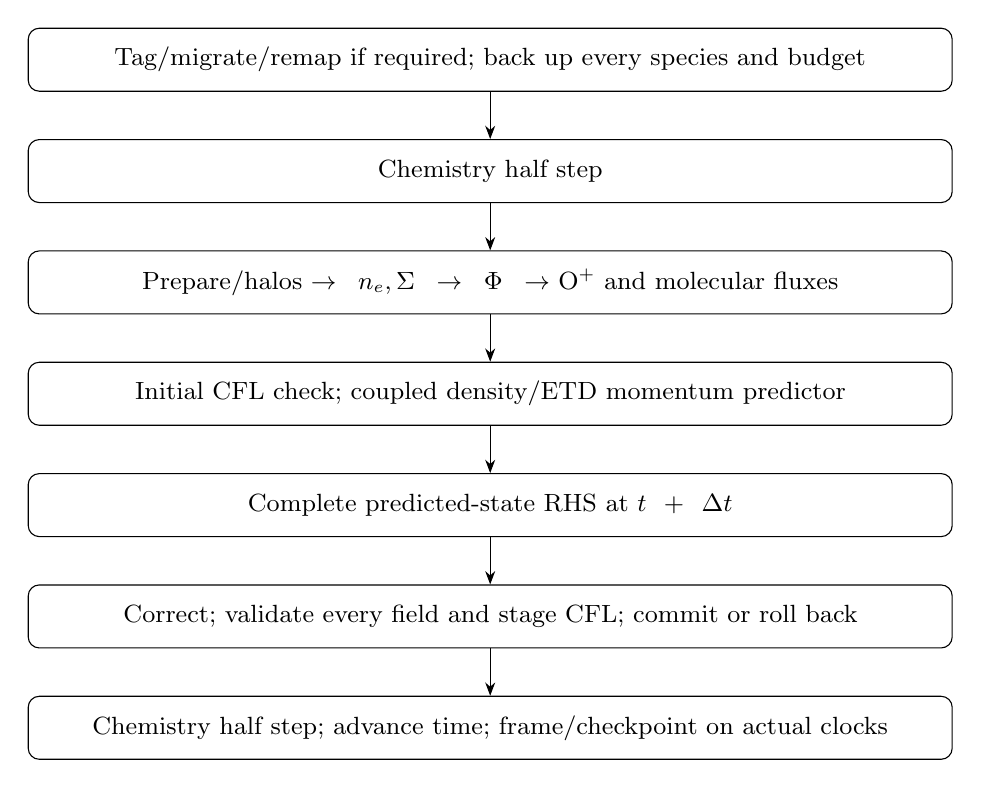
\begin{tikzpicture}[node distance=6mm,box/.style={draw,rounded corners,align=center,text width=115mm,minimum height=8mm,font=\small},>=Stealth]
\node[box] (a) {Tag/migrate/remap if required; back up every species and budget};
\node[box,below=of a] (b) {Chemistry half step};
\node[box,below=of b] (c) {Prepare/halos $\to n_e,\Sigma \to\Phi\to$ O$^+$ and molecular fluxes};
\node[box,below=of c] (d) {Initial CFL check; coupled density/ETD momentum predictor};
\node[box,below=of d] (e) {Complete predicted-state RHS at $t+\Delta t$};
\node[box,below=of e] (f) {Correct; validate every field and stage CFL; commit or roll back};
\node[box,below=of f] (g) {Chemistry half step; advance time; frame/checkpoint on actual clocks};
\foreach \x/\y in {a/b,b/c,c/d,d/e,e/f,f/g}\draw[->] (\x)--(\y);
\end{tikzpicture}
\caption{Actual coupled-step sequence. A smaller initial CFL proposal or failed
predictor/corrector restores all backed-up species and ledgers.}
\end{figure}

\subsection{Stability, retries and clocks}
The transport stability estimate is an owner-volume maximum of accumulated
absolute perpendicular volume flux plus parallel characteristic/fitted
rates divided by volume. Molecular rates are included in the same global
maximum. Initial dt is bounded by $0.9\,\mathrm{CFL}/r$, dt maximum, stop
time, output time, driver knot and maximum regrid clock. The predicted stage
must satisfy $\Delta t r^{(1)}\le\mathrm{CFL}(1+10^{-12})$.

Half-step chemistry can change the actual initial-stage rate. If its
post-chemistry CFL dt is smaller, the implementation restores the entire
pre-attempt state and repeats chemistry/RHS at the smaller dt. This path
is counted as an \emph{initial CFL adjustment}, separately from
predictor/corrector failure retries that halve dt. At most24 attempts are
allowed; failure or dt below $10^{-12}$ s is fatal. The new counters make
this extra work visible. A remesh resets the rate until an actual transport
evaluation, so proposal quality after regridding remains an optimization
opportunity; this release does not weaken the stability criterion to hide it.

Initial/final frames are always written. Reported physical time is the
actual accepted clock. A final saved field is never artificially held
while its movie label advances. Output and regrid intervals are independent
of physical forcing timescales.

\section{Adaptive density and potential approximations}
\subsection{Physical levels, segmented activity and backing storage}
The adaptive hierarchy has transverse refinement ratio2. For user roots
$N_x\times N_y$, two physical levels have canonical dimensions
$2N_x\times2N_y\times N_\parallel$; three have
$4N_x\times4N_y\times N_\parallel$. The implementation doubles its internal root
dimensions for three levels, so private levels $-1,0,1$ correspond to
physical L0,L1,L2. This is an anisotropic flux-tube/slab hierarchy, not a
general three-dimensional octree: $N_\parallel$ does not change.

Density refinement can vary with the along-field index, promoted over
\code{amr-slab-cells} neighboring segments. A column union supports any
fine density segment or electric-field request. Only the actual density
owner evolves at each $k$; other backing slots have zero owner volume.
Virtual children remain available to reconstruction. In a three-level
coarse macro volume, one primary backing slot represents four internal
root volumes. Hanging potential nodes obey a separately constrained
transverse approximation space. Thus active density cells, backing slots,
potential DOFs and canonical samples are different counts.

\begin{figure}[ht]
\centering
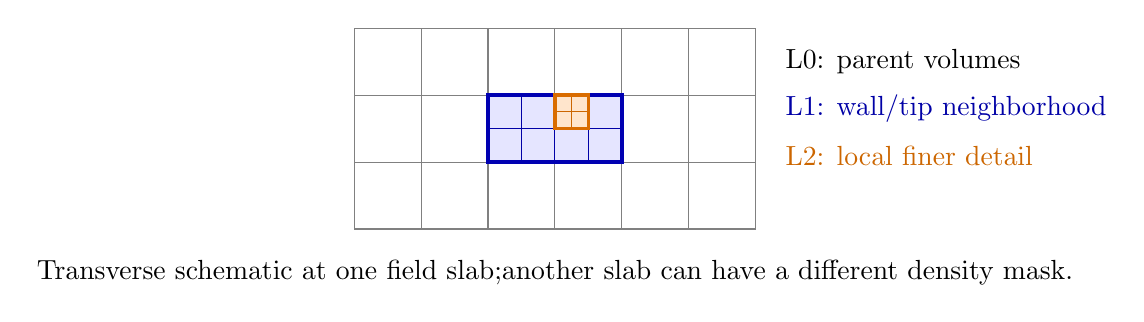
\begin{tikzpicture}[scale=.85]
\draw[step=1,gray] (0,0) grid (6,3);
\fill[blue!10] (2,1) rectangle (4,2);
\draw[step=.5,blue!65!black] (2,1) grid (4,2);
\fill[orange!20] (3,1.5) rectangle (3.5,2);
\draw[step=.25,orange!80!black] (3,1.5) grid (3.5,2);
\draw[very thick,blue!70!black] (2,1) rectangle (4,2);
\draw[very thick,orange!85!black] (3,1.5) rectangle (3.5,2);
\node[anchor=west] at (6.3,2.5) {L0: parent volumes};
\node[anchor=west,blue!65!black] at (6.3,1.8) {L1: wall/tip neighborhood};
\node[anchor=west,orange!80!black] at (6.3,1.1) {L2: local finer detail};
\node[align=center] at (3,-.65) {Transverse schematic at one field slab;\newline
another slab can have a different density mask.};
\end{tikzpicture}
\caption{Illustrative hierarchy only, not an image of a saved plasma solution.
The actual masks are output at each frame. Proper nesting and buffers are
computed from the detector, not prescribed by this sketch.}
\end{figure}

\subsection{Conservative restriction and prolongation}
Restriction preserves number and signed parallel momentum:
\begin{equation}
 N_P=\frac{\sum_cV_cN_c}{V_P},\qquad
 M_P=\frac{\sum_cV_cM_c}{V_P},\qquad V_P=\sum_cV_c.
\end{equation}
For prolongation, fit a local background amplitude $A$ using neighboring
parent differences and the existing reference basis $B$. Write child
density as a background-shaped part plus a residual and transverse slopes.
Logical child offsets are centred by volume weights, ensuring zero
volume-weighted slope correction. Bounds and a common positivity factor
limit the slopes without changing the parent average. The special
proportional-background branch avoids artificial cancellation residuals
when true child densities are many orders below a parent mean.

Parallel velocity is reconstructed separately. Its child slope correction
is centred using \emph{particle} weights $V_cN_c$, not merely volume,
so $\sum V_cN_cu_c=V_PM_P$. Applying a volume-centred velocity correction
would in general violate momentum conservation when density varies.
The optional seed marker follows the same particle-consistent transfer.
Remap verifies global particle, signed momentum and tracer invariants with
the original states retained until migration and transfer finish.

\subsection{Density residual, gradient and curvature criteria}
For a local $3\times3$ transverse stencil let
$n_0$ be its centre and
$n_{\rm norm}=\max(10^{-3}N_{\rm scale},\max n_{uv})$.
Raw first and second logical differences give
\begin{equation}
 G=\max(|D_xn|,|D_yn|)/n_{\rm norm},\quad
 C=\sqrt{D_{xx}^2+D_{yy}^2+2D_{xy}^2}/n_{\rm norm}.
\end{equation}
The normalization scale is strictly a detector scale; it is not inserted
into densities or the potential coefficient.

In represented-background mode, the local coefficient is
\begin{equation}
 A=\frac{\sum_{d=1}^4(B_d-B_0)(n_d-n_0)}
          {\sum_{d=1}^4(B_d-B_0)^2},
\end{equation}
with zero when the denominator vanishes. Apply the differences instead to
$R_{uv}=(n_{uv}-n_0)-A(B_{uv}-B_0)$. This removes only what the current
background-preserving reconstruction can already represent. It neither
evolves an unperturbed control nor subtracts one from the physical state.
Density walls, tips and branches can therefore request resolution while
a quiet represented altitude gradient need not refine an entire domain.

Refine/keep thresholds differ: release qualification uses
$G_{\rm on/off}=0.125/0.0625$ and $C_{\rm on/off}=0.02/0.01$.
Fine child indicators are also inspected before coarsening; a smooth parent
average must not hide canceling child detail. Prospective-parent information
loss is
\begin{equation}
 L=\max_c|N_c-N_c^{\rm prospective}|/n_{\rm norm},
\end{equation}
where the prospective values use the production conservative prolongation.
$L>0.005$ retains refinement. Marker-bearing regions can use the tighter
$\min(0.005,0.1A_{\rm declared})$ bound.

\subsection{Velocity, conductivity and weak-seed protection}
The velocity criterion uses the Hessian norm of the current E-cross-B
drift, scaled by maximum tag interval divided by local physical spacing.
It therefore detects a dynamically developing tip or curvature even before
deep depletion forms. Its keep threshold is half the refine threshold.
Second differences of all four integrated conductivity tensor components
provide an independent \emph{field-space} request, also with half-threshold
hysteresis. That request need not refine density along the whole tube.

If seed protection is enabled, an advected material marker identifies
the protected envelope. The required declared seed wavelength is sampled
by at least 32 cells and the vertical envelope by at least 8 cells. Tagged
developing structure can invoke an additional declared branch wavelength.
Any location still unresolved at the available finest level is counted.
An amplitude cannot be recovered after a coarse initial mesh has erased it;
protect the shortest relevant early mode from initialization. The late-time
qualification explicitly disables historical seed-marker reconstruction
and retains the existing developed checkpoint state.

\subsection{Buffers, physical-time hysteresis and proper nesting}
Structure requests receive a transverse root-cell buffer and promotion over
the current along-field slab. There is no unconditional whole-tube OR of
density requests. Three-level macro requests include required parents around
fine requests, including slab contacts and corners. A previously refined
cell can coarsen only after both its quiet duration and residence duration
exceed the configured physical quiet time, 60 s in the qualification.
Zero-hold simultaneous coarsening remains outside the qualified policy.

A check is triggered by the maximum tag interval or earlier when accumulated
transverse travel reaches half an internal-root scale. Consequently a
30 s maximum interval can yield actual regrids every few seconds. The
time-based hysteresis prevents those frequent checks from immediately
removing recently added resolution. Buffers cover stencil support and
anticipated motion; they are not a prescription to refine a fixed rectangle
around all depleted cells.

The retained legacy detector uses a same-time upper-quartile longitude
reference, depletion/gradient thresholds and a quiet-check count. Its
policy differs from the production structure criterion; changing between
them is a changed numerical case, not a performance-only optimization.

\subsection{Conservation and relation to general AMR frameworks}
The hierarchy follows the need for conservative transfer, proper nesting
and consistent interface flux emphasized by established AMR methods
\citep{BergerColella,Stone2020,Toth2012}. Here all levels use the same
accepted time step and the same summed physical interface flux. There is
no subcycled flux register. The prescribed magnetic field is not evolved,
so MHD constrained-transport or divergence-preserving magnetic prolongation
does not apply. Importing an MHD refinement mechanism without these
distinctions would not specify an ESF method.

\section{MPI ownership and hybrid kernel safety}
\subsection{Root-row partition and migration}
The partition planner balances the cumulative row estimate
\begin{equation}
 W_j=\frac1{N_\parallel}\sum_{i,k}(1+3r_{ijk})+
 w_{\rm canonical}N_{x,\rm internal},
\end{equation}
where $r$ is the density fine mask and $w_{\rm canonical}=0.5$ in the
qualified case. Whole-row cuts approximate equal prefix work, then
three-level cuts align to pairs. The estimate does not fully model
macro coarsening, molecular chemistry cost or ghost work. With only 80
physical L0 rows, 64 MPI ranks necessarily have coarse granularity.

O$^+$ halos extend six internal rows per side for three levels and three
for two levels; molecular response halos have their own narrower slab
width. At 13500 s, reconstruction of the exact partition from saved masks
gives 48 ranks owning one L0 row and 16 owning two. The largest molecular
owned-cell count is 1.6 times the mean; the largest O$^+$ activity count is
about 1.658 times its mean. The arithmetic mean of per-rank O$^+$
ghost/backing-owned ratios is 5.219. These are work/storage counts, not
exclusive timing percentages or a predicted speedup.

Molecular state keeps global backing but only owned/valid ghost values may
be read during evolution. On repartition, old/new slab intersections
transfer only changed ownership into separate receive buffers. Old owned
values remain valid until all sends and O$^+$ remapping finish. Identical
ownership is a byte-preserving no-op. Full molecular gathers are reserved
for output/checkpoints.

\subsection{What OpenMP parallelizes}
Independent cell kernels include molecular response refresh, current-stage
pressure-log preparation, final pressure/source normalization, stage
updates and macro-cell chemistry. Each active O$^+$ volume maps to disjoint
canonical reaction cells. Workers accumulate private reaction/charge
diagnostics, followed by reductions. A worker does not call MPI or abort
through the MPI failure path; invalid states are reported to the main
thread first.

Molecular face traversal is parallel by whole nonintersecting grid lines:
all $x$ lines in one $j$ row, all $y$ lines in one $i$ column, and one $(j,i)$ field line for a field sweep. The field-coordinate index stays innermost and contiguous in memory. A line retains serial face order. Two workers cannot write the same
cell during one axis sweep, and axis sweeps are separated by barriers.
Only scalar budget reductions change summation order. Blindly threading
individual faces would race on both neighboring cells.

AMR O$^+$ face blocks remain on the main thread. Their different-sized
contacts and lazy \code{ready}/child reconstruction caches require a
separate ownership strategy. Likewise canonical electron reconstruction
calls lazy sampling and is not blindly threaded. All MPI/PETSc calls stay
on the main thread under FUNNELED support. The executable verifies the
provided MPI thread level for multiple workers.

\subsection{Placement and resource accounting}
Each rank must have an allowed CPU domain large enough for all workers;
one-core binding cannot support four effective workers. Qualification
checks actual thread counts, inherited affinity and disjoint same-node
rank masks. Rank/worker count, active threads and Slurm reserved CPUs are
reported separately. A 32-by-2 comparison has the same 64 active threads as
64-by-1; a 64-by-4 comparison has256 active threads even when both fit the
same previously reserved256-CPU allocation. Neither should be mislabeled
as a fourfold same-resource algorithmic speedup.

\section{Software architecture and reproducible execution}
\subsection{Module responsibilities and ownership contracts}
The command-line entry point validates input before constructing a model.
Omitting \code{--amr-mode} selects the uniform reference solver; specifying
\code{none}, \code{fixed}, \code{fine} or \code{dynamic} selects the AMR
backend. There is no literal \code{static} enum. PETSc is required by AMR;
the \code{--petsc-potential} selector separately controls the static backend.
The build may omit MPI/PETSc for geometry utilities and the small reference
solver. OpenMP is optional and requires the MPI/PETSc configuration.

\begin{longtable}{p{.25\linewidth}p{.68\linewidth}}
\toprule Module & Responsibilities and contracts \\ \midrule\endhead
\path{igrf.c},\newline\path{geometry.c}&Field evaluation, target/apex conversion,
 tracing, hexahedral metrics, prescribed conductivity responses.\\
\path{pdm.c},\newline\path{integrator.c}&Physical-volume reconstruction moments and
 limiter; stable exponential drag weights.\\
\path{amr3.c}&Coupled driver, face-block topology, O$^+$ transport, complete
 stage RHS, clocks, frame output and conservative static import.\\
\path{amr3_mesh.c}&Backing/owned/ghost layout, immutable-cache reuse,
 restrictions, lazy sampling, conservative transfer and invariant checks.\\
\path{amr3_macro.c}&Third physical level, macro ownership, virtual internal
 children, parent tags and nested field constraints.\\
\path{amr3_structure.c},\newline\path{amr3_tags.c}&Structure detector, reason bits,
 prospective-parent loss and marker protection; legacy detector dispatch.\\
\path{amr3_potential.c}&Full integrated tensor, constrained Galerkin/COO
 assembly, regional boundary terms and checked PETSc solves.\\
\path{amr3_adapt.c},\newline\path{amr3_migration.c}&Ownership planning, old/new
 intersections, conservative remap and post-remap potential.\\
\path{amr3_night.c},\newline\path{amr3_molecular.c}&Prescribed neutral/rate loading,
 reactions, common Ne, molecular fluxes/stages and complete rollback.\\
\path{night.c},\newline\path{night_transport.c}&Pure local rate/solar/mobility/fitted
 flux kernels with explicit units and vacuum branches.\\
\path{amr3_restart.c},\newline\path{amr3_checkpoint2.c},\newline\path{amr3_cache.c}&Portable
 state formats, physical/numerical signatures and native geometry cache.\\
\path{transport.c},\newline\path{potential.c},\newline\path{petsc_potential.c},\newline
\path{output.c},\newline\path{restart.c}&Uniform reference solver, its small or PETSc
 potential backend, output and static restart.\\
\path{neutral_grid.c},\newline\path{electric_driver.c}&Strict externally supplied
 neutral/collision data and time-dependent imposed field.\\
\bottomrule
\end{longtable}

The \code{A3} state holds configuration, mesh/partition, owner metrics,
reconstruction caches, PETSc objects, detector history and rank-local
counters. Its \code{current_n/current_m} are borrowed current-stage views.
\code{slot[global_column]} is $-1$ outside the local halo;
\code{global[local_slot]} reverses the valid map. Owned slots precede ghosts.
Copying the struct requires \code{a3_rebase} to repair pointers into its
embedded level-array storage. A shared-cache reference count keeps immutable
geometry/PDM tables alive across rebuilds. Per-mesh tables and PETSc objects
are separately destroyed. The molecular object distinguishes its global
canonical count from owned workspace count.

\subsection{Array layout and stage-validity map}
Canonical cell/node storage has the field-coordinate index contiguous.
Face-family dimensions include one extra entry only in the face-normal
direction. The distinction between globally allocated backing and locally
valid values is part of the algorithm, not a plotting convention.
\begin{longtable}{>{\raggedright\arraybackslash}p{.28\linewidth}p{.64\linewidth}}
\toprule Array group & Meaning and validity \\ \midrule\endhead
\code{leaf}, \code{first}, \code{row}, \code{cover}&Backing-column labels, root-to-first-column,
 row prefix and canonical-cover maps. Stable for one mesh epoch.\\
\code{slot}, \code{global}, \code{partition}&Global/local translation and contiguous owned
 root-row cuts. Rebuilt on changed ownership.\\
\code{metric}&Actual owner volume, collision, gravity, reference density
 and two parallel areas. Nonowner slots have zero volume after masking.\\
\code{root_volume}, \code{root_bg}, \code{fine_bg}&Immutable reference geometry/background
 shared across rebuilds; they are not current plasma density.\\
\code{response[12]}&Per canonical cell: indices0--3 O$^+$ tensor per
 normalized density,4--7 additional molecular tensor,8--9 O$^+$ gravity
 current and10--11 additional molecular current. Molecular parts refresh
 from current transported species when night mode is on.\\
\code{base_n}, \code{base_m}, \code{base_velocity}&Prepared internal-root views from actual
 owners; macro-coarse cells populate conservative virtual root children.\\
\code{ready}, \code{child_n}, \code{child_m}, \code{child_velocity}&Lazy reconstruction caches.
 Density and velocity validity are distinct; reset on each prepare.
 Concurrent sampling is not automatically safe.\\
\code{macro_mask}, \code{macro_state}&Actual L0 ownership and prepared macro
 density/momentum/velocity/marker views. Read only after restriction.\\
\code{ion}, \code{momentum}, \code{electron}&Full canonical molecular backing and common
 electron array; only owned/refreshed dependencies are valid during RHS.\\
\code{backup}, \code{old_n}, \code{old_m}, \code{dn}, \code{dm}&Owned molecular rollback, stage and RHS
 workspaces. All species roll back together on a rejected attempt.\\
\code{transport_log}, \code{etd_weight}&Current-RHS pressure logarithms and
 same-attempt drag coefficients. Neither may silently survive an invalidating
 density/dt/ownership change.\\
\code{electron_average}, \code{electron_ready}&Owned-only, lazy
volume-weighted Ne averages at private levels$-1,0,1$. Reset whenever
\code{a3_night_electrons} rebuilds the current electron state. Accessed on
the main thread, with the original direct calculation outside owned cells.\\
\code{map}, \code{COO}, \code{matrix}, \code{ksp}, \code{phi}&Constrained independent-to-canonical potential
 map, geometric assembly factors and current material solve.\\
\bottomrule
\end{longtable}
The source atlas prints the precise types, formulas and indexing of each
group. The strict input/output schema must be used instead of the in-memory
member order. Real MPI status buffers and explicit C11 array qualification
conversions eliminate vendor-header/pedantic diagnostics without suppressing
compiler checks or changing numerical arithmetic.

Every runtime function has an adjacent responsibility comment, with units
and state/collective caveats at module and structure definitions. The
function appendix provides all 299 runtime C definitions; the source atlas
also includes headers and tests. Short inline ownership helpers in the
internal header follow its explicit count/index contract.

\subsection{Cache validity and optimizations in this release}
The following changes preserve the physical inputs, limiter/CFL/residual
policies and output cadence of the qualification:
\begin{enumerate}
\item Three-level construction no longer builds raw metrics twice.
  \code{a3_macro_metrics} remains the sole reset/build path before applying
  segmented masks, including restart remasking.
\item Macro volume/background tables are copied from unchanged geometry
  rather than repeating four-child reductions on every rebuild. Separate
  table ownership is retained.
\item The two conversion half-operators within one reaction call reuse
  identical rate/duration exponential coefficients. Density-dependent
  recombination coefficients are still reevaluated.
\item Predictor/corrector reuse ETD weights only within one attempted dt.
  Zero drag uses the exact analytic limit. Current-stage pressure logs
  retain their earlier per-RHS validity policy.
\item Repeated O$^+$ pressure/fitted-flux requests reuse the same owned
  volume-weighted electron average within the current electron state. The
  first request retains the original summation and division, including the
  finest-level $n_eV/V$ expression. All readiness flags are cleared before
  rebuilding Ne; no average survives a stage change. Off-owner requests use
  the original calculation. These lazy cache writes remain on the main
  thread and are not introduced into worker loops.
\item Audited independent kernels use optional OpenMP; MPI/PETSc, lazy
  reconstruction and AMR O$^+$ face traversal retain main-thread ownership.
\item Call-reason counters expose initial CFL repeats separately from
  predictor/corrector failure retries.
\end{enumerate}
The previous qualified release already replaced unconditional full
molecular gathers during every regrid with owned-intersection migration,
removed unused O$^+$ logarithms and reused molecular pressure logarithms.
Those earlier gains are not counted a second time in the new paired result.
No \code{fast-math}, density floor, conductivity floor, velocity cap,
looser potential residual, reduced output or changed refinement threshold
is used to obtain a speedup.

Several arrays still have global backing and several loops still visit
inactive or ghost slots. A prospective active-index optimization must
retain virtual child data required by PDM and coarse/fine sampling.
Further two-dimensional/block ownership and molecular AMR are substantial
changes, not already implemented features of this frozen release.

\subsection{Input files, defaults and effective cases}
The complete 79-option reference in the appendix is generated from an
explicit documented set checked against the parser's literal options.
Executable defaults differ from teaching/qualification cases. For example,
the executable retains CFL 0.35 and residual request $10^{-9}$, whereas the
qualified case explicitly specifies 0.25 and $10^{-10}$. Scientific claims
must use the effective case, not an assumed default or historical README.

A height collision table contains height in metres and positive O/e
collision rates in $\mathrm{s^{-1}}$. A height neutral table contains
$h,n_O,n_{N2},n_{O2},T_n$ with SI neutral densities, positive values and
full-domain coverage. Log interpolation is used. A spatial \code{ESFNEU01}
input has dimensions, component count, exact canonical-position hash,
temperature pair, data hash and six values per cell: $n_O,n_{N2},n_{O2},T_n,
\nu_O,\nu_e$. It is frozen, not an internal MSIS evaluation. UTC is
independent of IGRF decimal year and is neither HKT nor MLT.

The example launcher reads checked-in JSON, resolves input paths, prints
the full command and applies only explicit requested overrides. It refuses
an output already containing run metadata. The 0.2 s smoke case verifies
workflow, not bubble development; the 600 s teaching cases are deliberately
small and not substitutes for resolved event simulations.

\subsection{Outputs and frame-to-mesh binding}
\code{frames.csv} binds each time to a saved state, potential, leaf layout
and metrics epoch. \code{structure_frames.csv} additionally records actual
activity, backing count, field DOFs, density mask and tag outputs.
\code{state} is float64$[2,n_{\rm leaf},N_\parallel]$ with O$^+$ $N,M$;
\code{display_density} is reconstructed canonical O$^+$, not electron
density. Molecular density/momentum each have shape
$[2,N_{y,f},N_{x,f},N_\parallel]$. Canonical Ne adds both species to reconstructed
O$^+$. \code{amr_level} uses actual physical level0/1/2. Tag bits are
gradient1, curvature2, velocity4, seed8, loss16, buffer32, hold64, field128
and represented-background256. The six tag values are $G,C,V,L,G_{\rm raw},
C_{\rm raw}$.

Saved leaf metrics contain volume, background, collision rate, gravity and
the two parallel areas in that explicit order, which differs from the C
struct member order. Never reinterpret a visualization file as a C struct.
Native visualization data require explicit format/endianness awareness;
portable checkpoint encoding is a separate contract. Reconstructed coarse
display detail is not independently evolved fine-scale plasma.

\subsection{Portable checkpoints and strict identity}
Absolute particle/mass ledgers integrate stored normalized density; multiply
them by $n_*=10^{12}\,\mathrm{m^{-3}}$ for physical particle numbers. They
are not kilograms. Momentum integrals additionally require the species mass
when interpreted as physical mass momentum. Relative conservation errors do
not depend on the normalization. Initial molecular total is calculated over
replicated canonical geometry and is not reduced a second time over ranks.

Native checkpoints use little-endian64-bit integers and IEEE doubles,
ordered signatures and a final FNV checksum. Magic identifies legacy
\code{ESFAMR01}, structure02, driver03, spatial-neutral04 and three-level05
extensions. Structure formats retain density/field masks, quiet/birth
clocks, optional tracer, state, potential, original mass/boundary history
and input/source identities. Different MPI ranks are supported through
reconstruction of the owned layout when the physical case is compatible.

The molecular \code{ESFNIT02} file carries a numerical-source ID and the
hash of the exact paired native file, followed by physical clocks,
temperature/history and species arrays. Each file is atomically replaced,
but the pair is not a two-file transaction: a checkpoint is complete only
when both agree. A stop between writes can leave two individually complete
but incompatible files. Archive only a verified pair.

\code{ESFGEO01} is a different, native-ABI geometry cache with input,
parameter, source, ABI-size and payload checks. Editing geometry comments
changes its raw source fingerprint. Such strict rejection is intentional;
do not turn it into a general bypass. The qualification alone converts
isolated historical test copies after token-parity proof, updating only
metadata/checksums while proving identical physical payloads. Runtime
identity checks remain unchanged. SHA256 release/input manifests complement
the noncryptographic FNV integrity checks.

\subsection{Build, tests and publication boundary}
CMake builds the geometry utilities, local kernels, uniform solver and
optional PETSc/AMR backend. The qualification uses C11, GCC 12.3, Intel
MPI 2021.3, PETSc 3.26.1 real-double, Release/O3 and LTO. Optional OpenMP
requires compiler/runtime support. Site account, modules and absolute
paths belong in external launch scripts, not physical defaults.

The release contains code, official coefficients, explicit small examples,
documentation, test sources, manifests and methods sources/PDFs. Large
historical checkpoints, native caches, observed ISR data and cluster-specific
credentials are not Git payloads. Publication of the teaching case therefore
does not imply distribution of every production restart dataset. The
provenance distinguishes exact run qualification from the separately
specified student workflows.

\section{Limitations and appropriate scientific use}
A successful numerical gate demonstrates its defined invariant, not all
physical conclusions. Source/field parity does not validate empirical
collision multipliers, a prescribed neutral bath, idealized seed location,
PRE/wind history or an ISR comparison. IGRF geometry does not automatically
calibrate a Hong Kong evening. The UTC clock and whole-conjugate E-region
illumination matter for any night interpretation. Long elapsed simulation
time can exceed the regime of a prescribed background even when the solver
continues stably.

Zero-hold simultaneous coarsening is outside the qualified configuration;
the released science cases retain 60 s quiet/residence time. General
octree AMR, molecular adaptivity, energy/neutral coupling, full reaction
momentum, molecular perpendicular pressure diffusion and broad topology
changes are future work. Current one-dimensional rank ownership has a
finite granularity limit, and replicated geometry/molecular backing makes
memory scale less favorably than active O$^+$ count. The complete annotated
source and explicit case evidence define the actual implementation boundary.

\section{Verification, qualification and performance methodology}
\subsection{Different questions require different evidence}
The release checks the following separately:
\begin{enumerate}
\item Local kernels: collision/rate units, positive reaction maps, charge
 ledger, Bernoulli/vacuum limits and exponential drag weights.
\item Geometry/reconstruction: traced magnetic geometry, mapped-volume
 moments, cubic reproduction and bounded face reconstruction.
\item Elliptic algebra: manufactured tensor potential, regional/periodic
 boundaries and the explicitly recomputed true residual.
\item Transport/AMR: constant tracer, shared contacts, conservative
 density/momentum remap and the three physical-level entry paths.
\item Ownership: simultaneous/cross-peer molecular migration, round trips,
 exact no-op behavior and preservation of old owned state through remap.
\item Integration: fresh four-worker three-level and night-chemistry
 workflows, plus AddressSanitizer/UndefinedBehaviorSanitizer checks.
\item A developed-state qualification: complete saved-field and actual
 density-mask parity over the same physical interval, with full-process
 wall timing and separate resource accounting.
\end{enumerate}
Passing one does not replace the others. A 0.2 s teaching workflow validates
entry, coupling and output, not nonlinear bubble growth. Morphology is not
established by a rank count, residual or matching diagnostic scalar.

\subsection{The developed-state paired case}
The qualification continues one verified native/molecular checkpoint at
13350 s to 13500 s. User physical roots are 64 by80 with 64 field segments;
the three-level canonical geometry is256 by320 by64. The field is IGRF-14
at 2025.0, apex-longitude centre112.25 degrees and span8 degrees, spherical
apex range250--1600 km and conjugate base90 km. The frozen case retains
PDM4 with $\beta=1$, CFL 0.25, dt maximum 2 s, potential request $10^{-10}$,
the same transported-night closure, neutral inputs, seed/driver history,
structure thresholds, buffer 1, slab 4 and quiet 60 s. Output/checkpoints are
every 150 s, including initial and final frames.

The reference is the previously qualified owned-migration/log-cache version,
not the older production implementation. Old/new metadata-only source
bindings are audited in isolated copies; all physical payload bytes remain
unchanged. Geometry/IGRF token parity justifies annotation-induced identity
rebinding, with original hashes retained. Runtime readers still enforce
their exact identities. This is a validation conversion, not a public
restart bypass.

Within each allocation, one reference 64-by-1 launch precedes optimized 64-by-1,
32-by-2 and64-by-4 launches. The same 256 CPUs are reserved on two nodes, but
the active thread totals are 64,64,64 and256. Affinity probes precede model
launches and are excluded from model timing. The immediate synchronous
wait includes process start, geometry/cache/state initialization, output,
checkpointing and actual MPI exit. No PMPI observer is preloaded in any
of these launches. This differs from the earlier separate PMPI-observed
qualification; its absolute times must not be mixed into a new ratio.

Each field/component is compared with
\begin{equation}
 \epsilon_\infty=\frac{\max|q-q_{\rm ref}|}{\max|q_{\rm ref}|},
\end{equation}
scaling momentum components independently. This is a global-amplitude
normalization, not pointwise relative error near zero. Complete densities,
momenta, potential and reconstructed display fields at both saved times
are checked, and physical AMR level maps must be byte-identical. Conservation
and true residual must independently satisfy their acceptance criteria.

\subsection{Measured release qualification}
\noindent\textbf{Frozen numerical source ID.} \nolinkurl{b876245d6051ff517b9121fd6644ecafd762d5ff55ef5c3965895b8edd264c5d}\par
The frozen candidate completed all listed gates with zero compiler warnings.
Table~\ref{tab:perf} reports the complete matched launches on one two-node,
256-reserved-CPU allocation.

\begin{table}[ht]
\centering\small
\begin{tabular}{lrrrrr}
\toprule Variant & MPI & Workers & Active & Full wait(s) & Ratio \\ \midrule
reference64 & 64 & 1 & 64 & 499.981 & 1.000 \\
optimized64 & 64 & 1 & 64 & 481.027 & 1.039 \\
hybrid32x2 & 32 & 2 & 64 & 537.712 & 0.930 \\
hybrid64x4 & 64 & 4 & 256 & 374.899 & 1.334 \\
\bottomrule
\end{tabular}
\caption{Complete 13350--13500 s launches, including initialization,
outputs/checkpoints and actual process exit. Ratio is reference time divided
by row time. Every row reserves 256 CPUs, but active thread totals differ.
One launch per row; no statistical uncertainty estimate.}\label{tab:perf}
\end{table}

The same-active-thread64-by-1 implementation edit reduces full wait by
3.8\%. The fastest measured variant is
\code{hybrid64x4}, with 256 active threads; its
1.334 ratio is not a same-active-core algorithmic speedup.
The 32-by-2 configuration is slower than64-by-1 on this grid.
All saved-field checks pass; the largest global-amplitude-normalized
error is $6.765\times10^{-13}$, and actual AMR maps are byte-identical at both
frames. Completed true-residual and O$^+$ conservation checks also pass.
The new rank0 counters expose 400 accepted steps, 799 attempts, 399
initial CFL adjustments, 1200 RHS calls, 1199 chemistry calls and 41 tag
checks, with zero reported predictor/corrector failure retries. These
counts begin after the initial snapshot and include terminal diagnostic
RHS work. The release retains the stability/retry policy.

The exact source/build/input hashes, effective parameters, per-field errors
and completed diagnostics are recorded in \path{validation/qualification.json}.
Earlier separately paired candidate measurements are retained as history,
not mixed into the current speed ratio.


\begin{figure}[ht]
\centering
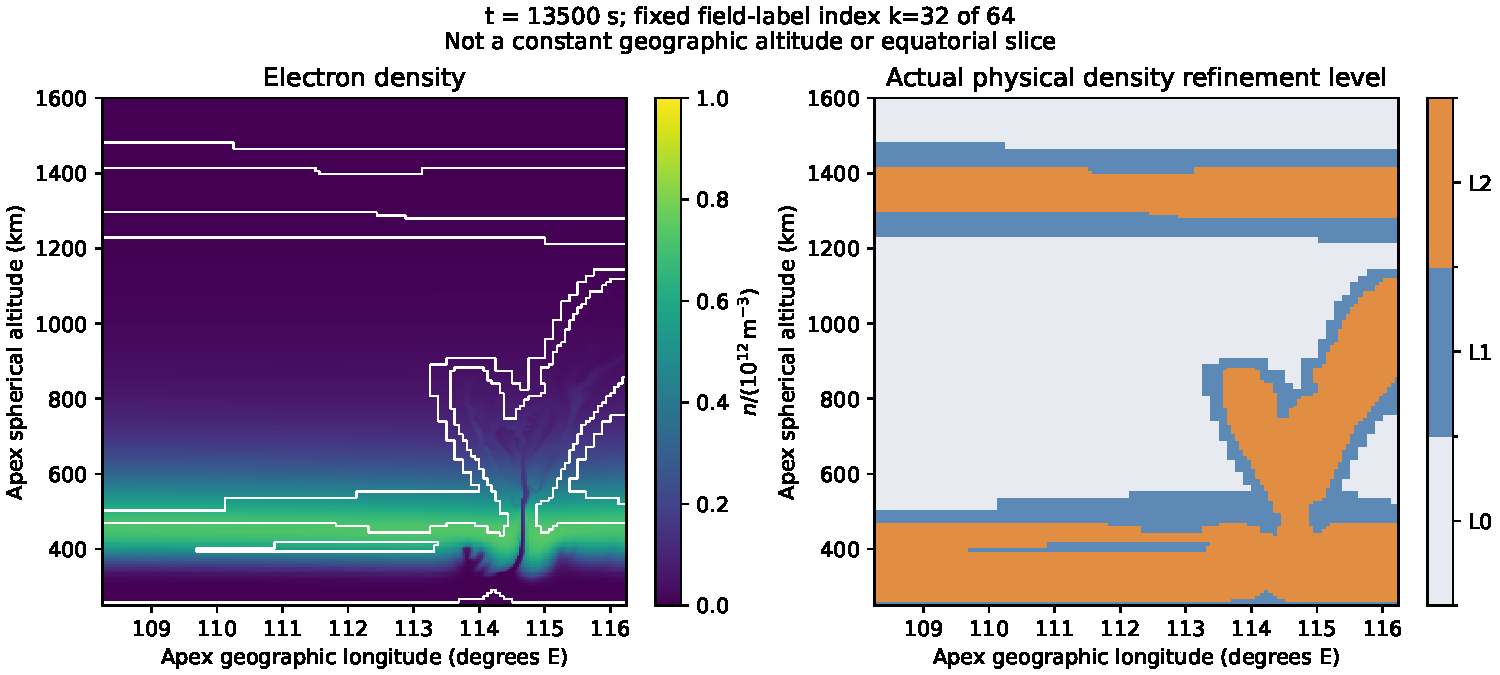
\includegraphics[width=\linewidth]{images/qualified_slice.pdf}
\caption{Saved 13500 s electron density and actual physical density-refinement
levels from the qualified 64-by-1 candidate. This is a fixed field-label-index
slice ($k=32$ of 64) plotted against apex longitude and spherical apex altitude;
it is neither an equatorial plane nor a constant geographic altitude cut.
Ne includes both molecular species. White digital cell-edge outlines separate
actual physical refinement levels; individual fine-grid cells are omitted.
Canonical O$^+$ detail in coarse regions is conservative display reconstruction,
not an independently evolved fine degree of freedom. Colors are clipped at
$10^{12}\,\mathrm{m^{-3}}$ for display only. Input/plot hashes and library versions
are recorded with the figure. No model integration was repeated to create it.}
\label{fig:saved-state}
\end{figure}

\subsection{Timing scope and retained failures}
Completion phase counters are rank-local and overlap: regrid includes
prepare/solve, and the legacy chemistry timer includes response refresh
and molecular halo wait. Terminal diagnostic RHS can be included in those
counters while the evolution interval timer ends before the last snapshot.
They are not an exclusive additive timeline. Independent phase maxima
must not be subtracted to claim an optimization. GNU-time CPU usage can
include MPI busy waiting and does not prove useful load balance.

Single paired launches have no repeated-run uncertainty estimate and are
not extrapolated to 20000 s production wall time. Increasing active workers
is distinguished from same-active-thread code/decomposition gains. All
successful states, failed gates/submissions and logs are preserved. A
reader/plot repair uses saved outputs rather than replaying a successful
scientific process. Production jobs and their controller are independent
of these isolated short qualifications and are not interrupted or modified.

\subsection{Evidence still needed for scientific publication}
This methods release does not claim a measured convergence order or exact
TELF validation, and none is inferred from PDM4's cubic stencil. Suitable
science studies should establish resolution sensitivity of the actual
depletion/branch observables, background/driver sensitivity, domain and
boundary influence, and observation sampling on actual ECEF geometry.
Hong Kong/Sanya ISR comparisons require electron rather than O$^+$ density,
appropriate height/beam coverage, correct local-time interpretation and
event-specific background provenance. Those studies are distinct from
demonstrating that a performance edit preserves an existing computation.

\bibliographystyle{plainnat}
\bibliography{references}
\appendix
\section{Complete command-line reference}
Actual executable defaults are listed here; explicit teaching and qualification cases differ. Every option except help takes one value.
\begin{description}[style=nextline,leftmargin=0pt,labelindent=0pt,labelwidth=0pt,labelsep=0pt]
\item[\texttt{--help}] \textit{Type/units: flag; default: n/a.} Print the short help and exit; this full reference includes extension options absent from short help.
\item[\texttt{--field}] \textit{Type/units: enum; default: igrf.} igrf: degree13; dipole: actual degree1 Gauss coefficients; aligned-dipole: axis-aligned fixture with specified equatorial strength.
\item[\texttt{--year}] \textit{Type/units: decimal year; default: 2025.} Coefficient interpolation epoch, 1900-2030; independent of the chemistry UTC clock.
\item[\texttt{--coeff}] \textit{Type/units: path; default: build-source data/igrf14coeffs.txt.} Official IGRF-14 coefficient file; pass a repository-relative or absolute path explicitly for relocatable runs.
\item[\texttt{--lon-deg}] \textit{Type/units: degrees east; default: trace HK350km apex.} Geographic APEX longitude at domain centre, not geographic longitude at HK350km. Automatic target is geodetic22.3N114.2E350km.
\item[\texttt{--span-deg}] \textit{Type/units: degrees; default: 2.5.} Total apex-longitude width, positive and <=20.
\item[\texttt{--nx}] \textit{Type/units: integer; default: 24.} User physical L0 longitude cells; >=4 and <=512, subject to canonical size limits.
\item[\texttt{--ny}] \textit{Type/units: integer; default: 40.} User physical L0 apex-height cells; >=4 and <=512. Three-level MPI rank count cannot exceed this value.
\item[\texttt{--ns}] \textit{Type/units: integer; default: 64.} Whole-conjugate along-field segments, 16-1024; never refined by transverse AMR.
\item[\texttt{--apex-min-km}] \textit{Type/units: km; default: 250.} Lowest tube apex spherical altitude; must exceed base altitude.
\item[\texttt{--apex-max-km}] \textit{Type/units: km; default: 1600.} Highest tube apex spherical altitude, above minimum and <=3000.
\item[\texttt{--base-km}] \textit{Type/units: km; default: 90.} Both conjugate endpoints at spherical altitude above6371.2km radius; 80-150.
\item[\texttt{--trace-step-km}] \textit{Type/units: km; default: 10.} Maximum RK4 tracing step, 0.1-20; tracing also reduces steps near the base.
\item[\texttt{--geometry-only}] \textit{Type/units: 0/1; default: 0.} Construct/load geometry and return before plasma evolution on AMR path.
\item[\texttt{--geometry-cache}] \textit{Type/units: path; default: none.} Native-ABI canonical geometry cache; exact parameter/input/code/ABI matching required.
\item[\texttt{--background-profile}] \textit{Type/units: enum; default: single.} single: Chapman peak438km scale70km; telf: sum of O+ Chapman populations with peaks438/600km, scales80/200km, relative amplitudes1/.01.
\item[\texttt{--E-peak}] \textit{Type/units: m\textasciicircum{}-3; default: 1e10.} Initial physical molecular E population, peak110km scale12km. Fixed without night module; initially NO+ with night module.
\item[\texttt{--amplitude}] \textit{Type/units: fraction; default: 0.1.} Seed fractional amplitude; absolute value <1. Positive values make a depletion in the configured envelope.
\item[\texttt{--seed-height-km}] \textit{Type/units: km; default: 350.} Spherical-altitude seed envelope centre.
\item[\texttt{--seed-width-km}] \textit{Type/units: km; default: 70.} Positive vertical seed envelope width; see exact initialization equation in methods.
\item[\texttt{--seed-east-km}] \textit{Type/units: km; default: 0.} Nonnegative horizontal seed width; zero selects the alternate wavelength pattern, not an eastward displacement.
\item[\texttt{--seed-lon-deg}] \textit{Type/units: apex degrees; default: domain centre.} Seed apex longitude, strictly inside the regional domain; explicit setting is incompatible with periodic-x.
\item[\texttt{--temperature-sum}] \textit{Type/units: K; default: 2500.} Fixed Ti+Te used by O+ parallel pressure/sound speed. Night module requires exact consistency with chem-Ti+chem-Te.
\item[\texttt{--dipole-equator-nT}] \textit{Type/units: nT; default: 31200.} Aligned-dipole equatorial amplitude; positive; does not replace all coefficients in ordinary degree-one dipole mode.
\item[\texttt{--parallel}] \textit{Type/units: 0/1; default: 1.} Include field-aligned transport/momentum. Zero is a deliberately reduced physical case.
\item[\texttt{--parallel-order}] \textit{Type/units: 1 or2; default: 1.} Order of the bounded along-field face reconstruction; distinct from transverse PDM4.
\item[\texttt{--parallel-flux}] \textit{Type/units: enum; default: rusanov.} rusanov or relaxation. Night module requires relaxation; includes collision/pressure/gravity fitted mass flux.
\item[\texttt{--exb-scheme}] \textit{Type/units: enum; default: muscl static; pdm4 AMR.} muscl or pdm4; explicit selection is recommended. PDM4 is a four-cell volume-moment cubic stencil with limiter.
\item[\texttt{--pdm-beta}] \textit{Type/units: dimensionless; default: 1.} PDM limiter correction bound2*beta*upstream difference; supported0-10. beta=0 reduces to donor-cell at the limiter.
\item[\texttt{--hall}] \textit{Type/units: 0/1; default: 1.} Retain integrated Hall conductivity cross terms; disabling changes physics.
\item[\texttt{--periodic-x}] \textit{Type/units: 0/1; default: 0.} Longitude periodicity; physical branch requires aligned dipole, zero imposed E and no localized horizontal seed.
\item[\texttt{--regional-x}] \textit{Type/units: 0/1; default: 1.} Regional open longitude particle boundary and polarization d\_xi(phi)=0 side condition; this is NOT zero total normal current.
\item[\texttt{--open-apex}] \textit{Type/units: 0/1; default: 0.} Open particle boundaries at transverse apex-height extremes; required for external driver cases.
\item[\texttt{--open-ends}] \textit{Type/units: 0/1; default: 0.} Open particle boundaries at both along-field endpoints; otherwise reflective/closed.
\item[\texttt{--background-east-mVm}] \textit{Type/units: mV/m; default: 0.} Prescribed constant eastward electric field, added through mapped potential; excludes CSV driver. AMR driver requires regional nonperiodic and open-apex geometry.
\item[\texttt{--electric-driver}] \textit{Type/units: CSV path; default: none.} time\_s,east\_V\_m strictly increasing from0 with coverage through absolute end; stage interpolation and step landing on knots.
\item[\texttt{--petsc-potential}] \textit{Type/units: 0/1; default: 0.} PETSc backend for uniform reference path. AMR inherently requires PETSc even though this static-path selector defaults0.
\item[\texttt{--rtol}] \textit{Type/units: dimensionless; default: 1e-9.} Requested true potential infinity-residual scale; positive and <.01; AMR accepts <=1.05*rtol after explicit residual computation.
\item[\texttt{--cfl}] \textit{Type/units: dimensionless; default: 0.35.} Positive and <=.45; initial proposal uses0.9*cfl/rate and stage acceptance uses cfl. Teaching/qualification cases explicitly use.25.
\item[\texttt{--dt-max}] \textit{Type/units: s; default: 2.} Positive maximum attempted step; all active levels/species share the accepted dt, with no subcycling.
\item[\texttt{--end}] \textit{Type/units: s; default: 3600.} Absolute elapsed-model stop time. On restart this is not additional duration.
\item[\texttt{--output-every}] \textit{Type/units: s; default: 600.} Positive frame/checkpoint interval; initial and final frames also written. Not a physics timescale or an AMR interval.
\item[\texttt{--max-steps}] \textit{Type/units: integer; default: 200000.} Absolute step counter limit, including history restored by restart.
\item[\texttt{--progress-steps}] \textit{Type/units: integer; default: 0.} Progress-print step interval; zero disables periodic progress lines but not essential diagnostics.
\item[\texttt{--out}] \textit{Type/units: directory; default: igrf\_run.} New run directory; an existing metadata.json is rejected to preserve prior outputs.
\item[\texttt{--restart}] \textit{Type/units: path; default: none.} Native AMR checkpoint or explicitly supported uniform-state import; physical/numerical signatures must match.
\item[\texttt{--night-restart}] \textit{Type/units: path; default: none.} Molecular ESFNIT02 paired with exact native checkpoint; required for night continuation.
\item[\texttt{--amr-mode}] \textit{Type/units: enum; default: unset = static reference.} none,fixed,fine,dynamic select the AMR backend. There is no literal static enum; omitting the option selects the uniform reference path.
\item[\texttt{--amr-levels}] \textit{Type/units: 2 or3; default: 2.} Number of PHYSICAL levels. Three requires structure criterion and nonzero along-field slab size.
\item[\texttt{--amr-case}] \textit{Type/units: enum; default: esf.} esf,translation,potential,remap. Latter three are verification fixtures, not physical ESF forecasts.
\item[\texttt{--amr-criteria}] \textit{Type/units: enum; default: legacy.} legacy percentile/depletion or structure local solution-based detector. Released examples explicitly select structure.
\item[\texttt{--amr-density-indicator}] \textit{Type/units: enum; default: total.} total or represented; represented removes a fitted local background-shaped component for detection only, never from evolved density.
\item[\texttt{--amr-slab-cells}] \textit{Type/units: integer; default: 0.} Along-field segment grouping for density tags. Zero means column-wide legacy layout; nonzero must divide ns and requires structure. Qualification uses4.
\item[\texttt{--amr-interval}] \textit{Type/units: s; default: 100.} Maximum tag-check interval. Accumulated transverse travel can trigger earlier checks; not a fixed actual regrid period.
\item[\texttt{--amr-buffer}] \textit{Type/units: integer; default: 2.} Transverse root-cell buffer around requested structure; 0-16. Qualification uses1.
\item[\texttt{--amr-work-weight}] \textit{Type/units: dimensionless; default: 0.5.} Additive canonical-field work estimate in root-row MPI partition planner; does not change physical equations.
\item[\texttt{--amr-coo}] \textit{Type/units: 0/1; default: 1.} Use cached constrained COO assembly; zero selects the reference element assembly algebra.
\item[\texttt{--amr-gradient-on}] \textit{Type/units: dimensionless; default: 0.08.} Refine threshold for normalized detector gradient; must be >=positive off threshold.
\item[\texttt{--amr-gradient-off}] \textit{Type/units: dimensionless; default: 0.04.} Lower keep-refined gradient threshold, providing spatial hysteresis.
\item[\texttt{--amr-curve-on}] \textit{Type/units: dimensionless; default: 0.02.} Refine threshold for normalized density Hessian norm.
\item[\texttt{--amr-curve-off}] \textit{Type/units: dimensionless; default: 0.01.} Lower keep-refined curvature threshold.
\item[\texttt{--amr-velocity-on}] \textit{Type/units: dimensionless; default: 0.1.} Threshold for interval-scaled drift curvature divided by local spacing; keep-refined threshold is half.
\item[\texttt{--amr-sigma-on}] \textit{Type/units: dimensionless; default: 0.05.} Integrated conductivity-tensor curvature threshold for FIELD requests, half when already refined.
\item[\texttt{--amr-quiet-seconds}] \textit{Type/units: s; default: 60.} Physical quiet and minimum residence time before coarsening; qualified production uses60. Zero-hold simultaneous coarsening is not qualified; see known limitations.
\item[\texttt{--amr-seed-guard}] \textit{Type/units: 0/1; default: 1.} Advect a material seed-protection marker and prevent under-resolved protected wavelengths. Fresh perturbed structure runs need explicit positive seed wavelength when enabled.
\item[\texttt{--amr-seed-wavelength-km}] \textit{Type/units: km; default: 0 = unspecified.} Shortest declared protected seed wavelength, not inferred from grid. Sampling target32 cells/wavelength; unresolved locations are reported.
\item[\texttt{--amr-branch-wavelength-km}] \textit{Type/units: km; default: 0 = disabled.} Additional protected wavelength when resolved walls/branches are tagged; zero disables this requirement.
\item[\texttt{--amr-seed-amplitude}] \textit{Type/units: fraction; default: 0.001.} Declared weak-seed amplitude used in protection/information-loss tolerance; distinct from density seeding amplitude.
\item[\texttt{--amr-deplete-on}] \textit{Type/units: ratio; default: 0.95.} Legacy detector depletion refinement threshold; below off threshold and positive.
\item[\texttt{--amr-deplete-off}] \textit{Type/units: ratio; default: 0.98.} Legacy keep-refined depletion threshold, <1. Not used as a density floor.
\item[\texttt{--amr-hold}] \textit{Type/units: check count; default: 2.} Legacy quiet-check count before coarsening; structure detector instead uses quiet-seconds.
\item[\texttt{--amr-fixture}] \textit{Type/units: enum; default: none.} none,flat,wall,tip,fork,weak synthetic detector fixtures; explicitly separate these from scientific seeding.
\item[\texttt{--night-chemistry}] \textit{Type/units: 0/1; default: 0.} Enable the full transported molecular module, not just local chemistry. Requires physical segmented structure AMR, neutral input, UTC, positive E peak and consistent temperatures.
\item[\texttt{--night-reactions}] \textit{Type/units: 0/1; default: 1.} With night module on, zero disables only reactions; NO+/O2+ still transport. It is not a fixed-reservoir switch.
\item[\texttt{--neutral-profile}] \textit{Type/units: path; default: none.} Five-column height table or strict spatial ESFNEU01 grid; physical values must cover the entire canonical conjugate geometry.
\item[\texttt{--collision-profile}] \textit{Type/units: CSV path; default: none.} height\_m,nu\_O\_s1,nu\_e\_s1; strictly increasing, positive and fully covering geometry. Without it use documented idealized analytic rates.
\item[\texttt{--utc-start-unix}] \textit{Type/units: Unix UTC s; default: 0 = unspecified.} Absolute UTC at model time0, required for night module; 2000-2100 range checked. Not HKT, LST or MLT.
\item[\texttt{--chem-Ti}] \textit{Type/units: K; default: 0 = unspecified.} Fixed ion temperature for all night species, 200-5000 and applicable reaction-fit range.
\item[\texttt{--chem-Te}] \textit{Type/units: K; default: 0 = unspecified.} Fixed electron temperature for night closure, 200-5000. Ti+Te must equal temperature-sum.
\end{description}

\section{Function-level implementation reference}
All runtime C definitions are bound to reviewed responsibilities and actual source lines. Units and cache/ownership contracts accompany the source. The complete implementation, headers and tests are in the separate source atlas.
\subsection{\texttt{src/amr3.c}}
AMR driver and conservative O+ fluxes. n is normalized by 1e12 m\textasciicircum{}-3; m=n*u\_parallel. Private levels -1/0/1 represent physical L0/L1/L2 in a three-level run.
\begin{description}[style=nextline,leftmargin=0pt,labelindent=0pt,labelwidth=0pt,labelsep=0pt]
\item[\texttt{wrap}] Return the nonnegative periodic index i modulo n. Source line 18.\par
{\small\nolinkurl{static int wrap(int i, int n)}}
\item[\texttt{cover}] Map a canonical transverse cell to its backing leaf column; apply the configured periodic/clamped indexing. Source line 26.\par
{\small\nolinkurl{static int cover(A3 *a, int i, int j)}}
\item[\texttt{owned}] Test whether a backing column belongs to this rank, so shared faces update only local conserved states. Source line 39.\par
{\small\nolinkurl{static int owned(A3 *a, int p)}}
\item[\texttt{ph}] Read a transverse potential node using this solver's boundary/periodic indexing convention. Source line 45.\par
{\small\nolinkurl{static double ph(A3 *a, int i, int j)}}
\item[\texttt{derivative}] Compute the two transverse potential derivatives at a geometric face and retain both metric cross contributions. Source line 52.\par
{\small\nolinkurl{static void derivative(A3 *a, int axis, int i, int j, double d[2])}}
\item[\texttt{minmod}] Return the sign-consistent slope with smallest magnitude; return zero at an extremum. Source line 78.\par
{\small\nolinkurl{static double minmod(double a, double b, double c)}}
\item[\texttt{length\_at}] Read the physical along-field segment length at the requested private refinement level. Source line 84.\par
{\small\nolinkurl{static double length_at(A3 *a, int level, int i, int j, int k)}}
\item[\texttt{cell\_value}] Sample density or velocity with the caller's parallel boundary convention; used by the along-field reconstruction. Source line 103.\par
{\small\nolinkurl{static double cell_value(A3 *a, int p, int k, int field)}}
\item[\texttt{parallel\_state\_at}] Construct a bounded left/right parallel face state at an explicitly requested refinement level. Source line 112.\par
{\small\nolinkurl{static double parallel_state_at(A3 *a, int level, int i, int j, int k, int field, int side)}}
\item[\texttt{parallel\_state}] Resolve the actual local density level, then reconstruct its parallel face state. Source line 122.\par
{\small\nolinkurl{static double parallel_state(A3 *a, int p, int k, int field, int side)}}
\item[\texttt{length}] Resolve a backing cell's active density level before reading its physical parallel length. Source line 129.\par
{\small\nolinkurl{static double length(A3 *a, int p, int k)}}
\item[\texttt{log\_pressure}] Compute the nonuniform parallel logarithmic pressure gradient, using common Ne in the multi-ion closure and exact-vacuum secants. Source line 137.\par
{\small\nolinkurl{static double log_pressure(A3 *a, int p, int k)}}
\item[\texttt{bernoulli}] Evaluate the Bernoulli fitting function z/(exp(z)-1) with small-argument series and large-argument limits. Source line 167.\par
{\small\nolinkurl{static double bernoulli(double z)}}
\item[\texttt{parallel\_cache}] Prepare shared parallel flux/rate tables for a column-uniform density layout; segmented layouts use a different path. Source line 182.\par
{\small\nolinkurl{static void parallel_cache(A3 *a, double cs)}}
\item[\texttt{density\_cover}] Locate the actual density owner at a canonical cell and along-field index; owner can differ from electric-field backing. Source line 246.\par
{\small\nolinkurl{static int density_cover(A3 *a, int i, int j, int k)}}
\item[\texttt{append\_face}] Append or merge a canonical face interval whose two active density owners and levels are unchanged. Source line 260.\par
{\small\nolinkurl{static void append_face(A3 *a, int axis, int i, int j, int first, int last)}}
\item[\texttt{a3\_face\_topology}] Build conservative face blocks for the current segmented density mesh; identical interface fluxes are shared by both adjacent volumes. Source line 299.\par
{\small\nolinkurl{void a3_face_topology(A3 *a)}}
\item[\texttt{metric\_at}] Read or conservatively aggregate geometry for a requested physical density level, including the macro level. Source line 332.\par
{\small\nolinkurl{static void metric_at(A3 *a, int level, int i, int j, int k, A3Metric *m)}}
\item[\texttt{a3\_parallel\_geometry}] Cache static segment lengths and parallel relaxation factors for every supported level. Source line 348.\par
{\small\nolinkurl{void a3_parallel_geometry(A3 *a)}}
\item[\texttt{segmented\_parallel}] Evaluate parallel particle/momentum flux for one actual segmented interface; retain collisional relaxation and electron-pressure fitting. Source line 389.\par
{\small\nolinkurl{static void segmented_parallel(A3 *a, int level, int i, int j, int k, double cs, double *N, double *M, double *rate)}}
\item[\texttt{marker\_fraction}] Return a bounded material seed fraction from the advected marker and density; zero density gives zero fraction. Source line 453.\par
{\small\nolinkurl{static double marker_fraction(A3 *a, int level, int axis, int i, int j, int k, int sign)}}
\item[\texttt{a3\_transport}] Compute O+ finite-volume density/momentum RHS, shared face fluxes, gravity/pressure sources and global stability/travel rates. Collective; sampling may populate lazy caches, so AMR face loops remain on the main thread. Source line 464.\par
{\small\nolinkurl{void a3_transport(A3 *a, double *dn, double *dm)}}
\item[\texttt{rhs}] Execute the complete current-stage chain: prepare/halo, integrated potential solve, O+ transport, then molecular transport. The potential always belongs to this stage's density and chemistry state. Source line 640.\par
{\small\nolinkurl{static void rhs(A3 *a, double *n, double *m, double *dn, double *dm, double time)}}
\item[\texttt{node\_id}] Flatten node coordinates with the along-field coordinate contiguous. Source line 652.\par
{\small\nolinkurl{static int node_id(TubeGrid *g, int i, int j, int k)}}
\item[\texttt{make\_box}] Build Cartesian synthetic geometry for transport/potential verification rather than tracing a physical magnetic field. Source line 659.\par
{\small\nolinkurl{static void make_box(TubeGrid *g, GridConfig c)}}
\item[\texttt{gather\_geometry}] Collect disjoint computed geometry row ranges into replicated canonical geometry, in MPI-count-safe chunks. Source line 700.\par
{\small\nolinkurl{static void gather_geometry(A3 *a, void *data, int rows, size_t rowbytes, const int *cuts)}}
\item[\texttt{parallel\_geometry}] Distribute tube tracing and cell/face metric construction among ranks, then assemble the replicated geometry and diagnostics. Source line 717.\par
{\small\nolinkurl{static void parallel_geometry(A3 *a, TubeGrid *g, Igrf *field, GridConfig fine)}}
\item[\texttt{geometry}] Load and validate a geometry cache, or construct geometry and optionally write a new cache; initialize conductivity responses afterward. Source line 772.\par
{\small\nolinkurl{static void geometry(A3 *status, TubeGrid *g, Config3 c)}}
\item[\texttt{output}] Open a named output in the current run directory; failures are collective-fatal through a3\_fail. Source line 833.\par
{\small\nolinkurl{static FILE *output(A3 *a, const char *name, const char *mode)}}
\item[\texttt{metadata}] Write effective geometry, numerical controls, units and binary layout metadata for this AMR run. Source line 845.\par
{\small\nolinkurl{static void metadata(A3 *a)}}
\item[\texttt{snapshot}] Collect owned states, reconstruct canonical display density, and write time/mesh-bound outputs plus the native checkpoint. Display reconstruction is not an evolved finest-grid solution. Source line 920.\par
{\small\nolinkurl{static void snapshot(A3 *a, double *n, double *m, int frame, double time, int step, double mass0, const int *quiet, double next_regrid, double travel, int retries)}}
\item[\texttt{remap\_tests}] Exercise constant/background/smooth conservative transfers and validate particle/momentum invariants in the dedicated remap case. Source line 1105.\par
{\small\nolinkurl{static void remap_tests(A3 *base, TubeGrid *g)}}
\item[\texttt{import\_static}] Import a uniform-grid restart by preserving original coarse-cell particle and signed momentum integrals on the canonical AMR geometry. Source line 1198.\par
{\small\nolinkurl{static void import_static(A3 *a, TubeGrid *g, double *n, double *m, double *time, int *step, double *mass0)}}
\item[\texttt{workspace}] Replace scratch arrays after a mesh rebuild so their sizes match the new owned-plus-halo backing layout. Source line 1285.\par
{\small\nolinkurl{static void workspace(A3 *a, double ***arrays, int count)}}
\item[\texttt{amr3\_run}] Drive initialization/restart, regridding, half chemistry, two-stage O+/molecular transport, acceptance checks, diagnostics and checkpointing. All ranks follow the same clocks; no level subcycling is used. Source line 1296.\par
{\small\nolinkurl{int amr3_run(Config3 c, int rank, int size)}}
\end{description}
\subsection{\texttt{src/amr3\_adapt.c}}
Collective mesh rebuild, ownership migration and conservative transfer. Geometry remains fixed; density and electric-potential approximation spaces may change separately.
\begin{description}[style=nextline,leftmargin=0pt,labelindent=0pt,labelwidth=0pt,labelsep=0pt]
\item[\texttt{migrate}] Transfer O+ density/momentum/optional marker intersections between old and new rank-owned slabs before conservative remapping. Source line 16.\par
{\small\nolinkurl{static void migrate(A3 *old, A3 *moved, double *n, double *m, double *N, double *M)}}
\item[\texttt{a3\_adapt}] Detect actual mask/field-space changes, repartition molecules and O+, build/remap the new mesh, verify global invariants and resolve potential. A no-change request returns without rebuilding. Source line 47.\par
{\small\nolinkurl{int a3_adapt(A3 *a, double **n, double **m, const unsigned char *mask, double time, int step, int exact_initial)}}
\end{description}
\subsection{\texttt{src/amr3\_cache.c}}
Native-ABI geometry cache. This is a performance cache, not a portable state checkpoint. Source/input identities, ABI sizes and payload checksum must all match.
\begin{description}[style=nextline,leftmargin=0pt,labelindent=0pt,labelwidth=0pt,labelsep=0pt]
\item[\texttt{hash}] Update the FNV-1a checksum over an exact byte sequence. Source line 20.\par
{\small\nolinkurl{static uint64_t hash(uint64_t h, const void *data, size_t n)}}
\item[\texttt{file\_hash}] Hash an input file for cache identity; an empty optional path has identity zero. Source line 31.\par
{\small\nolinkurl{static uint64_t file_hash(A3 *a, const char *path)}}
\item[\texttt{a3\_geometry\_identity}] Accept the exact compiled geometry identity or one explicitly enumerated, version-guarded historical equivalence; reject unknown changes. Source line 51.\par
{\small\nolinkurl{int a3_geometry_identity(A3 *a, const char code[128])}}
\item[\texttt{a3\_geometry\_cache}] Read/write native canonical geometry with complete parameter/input/source/ABI checks, atomic rename and payload checksum. Source line 88.\par
{\small\nolinkurl{int a3_geometry_cache(A3 *a, TubeGrid *g, Config3 c, int write)}}
\end{description}
\subsection{\texttt{src/amr3\_checkpoint2.c}}
Structure-aware ESFAMR02/03/04/05 checkpoint formats. Preserve density/field masks, hysteresis clocks, optional seed tracer and conservation history.
\begin{description}[style=nextline,leftmargin=0pt,labelindent=0pt,labelwidth=0pt,labelsep=0pt]
\item[\texttt{bytes}] Read or write exactly the requested bytes while updating the checkpoint checksum; short transfers are fatal. Source line 25.\par
{\small\nolinkurl{static void bytes(Stream *s, void *p, size_t n)}}
\item[\texttt{integer}] Encode/decode an unsigned 64-bit integer in little-endian order and update the stream checksum. Source line 38.\par
{\small\nolinkurl{static uint64_t integer(Stream *s, uint64_t value)}}
\item[\texttt{reals}] Transfer floating data in portable little-endian order, retaining the checksum over the actual encoded bytes. Source line 52.\par
{\small\nolinkurl{static void reals(Stream *s, double *p, size_t n)}}
\item[\texttt{finish}] Write or verify the final checksum, reject trailing data on reads, and close the checkpoint stream. Source line 68.\par
{\small\nolinkurl{static void finish(Stream *s)}}
\item[\texttt{parameters}] Choose the exact restart signature length required by this case's driver/neutral extensions. Source line 80.\par
{\small\nolinkurl{static int parameters(Config3 c)}}
\item[\texttt{signature}] Build the ordered physical/numerical restart signature; changing a signed parameter intentionally rejects incompatible restart. Source line 87.\par
{\small\nolinkurl{static void signature(Config3 c, double value[72])}}
\item[\texttt{a3\_checkpoint2\_write}] Atomically write structure-aware masks/history, optional tracer, actual conserved states, potential and checksummed physical/numerical signatures. Source line 127.\par
{\small\nolinkurl{void a3_checkpoint2_write(A3 *a, const double *n, const double *m, const double *marker, double time, int step, double mass0, double next_regrid, double travel, int retries)}}
\item[\texttt{a3\_checkpoint2\_read}] Validate and reconstruct a structure-aware checkpoint, distribute states under the current MPI decomposition, and restore mesh/clocks/history. Source line 206.\par
{\small\nolinkurl{int a3_checkpoint2_read(A3 *a, TubeGrid *g, Config3 c, int rank, int size, double **n, double **m, double *time, int *step, double *mass0, int **quiet, double *next_regrid, double *travel, int *retries)}}
\end{description}
\subsection{\texttt{src/amr3\_macro.c}}
Third physical level. A macro cell covers four internal roots. Only the primary backing slot evolves when its macro mask is coarse; volume-weighted virtual children serve reconstruction.
\begin{description}[style=nextline,leftmargin=0pt,labelindent=0pt,labelwidth=0pt,labelsep=0pt]
\item[\texttt{a3\_nx}] Return the transverse x dimension for a private level; level -1 is the extra physical coarse level. Source line 18.\par
{\small\nolinkurl{int a3_nx(const A3 *a, int level)}}
\item[\texttt{a3\_ny}] Return the transverse y dimension for a private level; level -1 is the extra physical coarse level. Source line 25.\par
{\small\nolinkurl{int a3_ny(const A3 *a, int level)}}
\item[\texttt{a3\_scale}] Return the number of canonical finest cells across one requested-level cell: 4, 2 or 1. Source line 31.\par
{\small\nolinkurl{int a3_scale(int level)}}
\item[\texttt{a3\_macro\_index}] Map an internal root index to its containing two-by-two macro cell. Source line 37.\par
{\small\nolinkurl{int a3_macro_index(const A3 *a, int b)}}
\item[\texttt{a3\_macro\_primary}] Return the unique backing column used to evolve an unrefined macro cell. Source line 43.\par
{\small\nolinkurl{int a3_macro_primary(const A3 *a, int b)}}
\item[\texttt{a3\_rebase}] Repair interior pointers after copying an A3 struct; they must point into the destination's own embedded storage. Source line 50.\par
{\small\nolinkurl{void a3_rebase(A3 *a)}}
\item[\texttt{coord}] Wrap or clamp macro coordinates according to physical versus synthetic boundary policy. Source line 59.\par
{\small\nolinkurl{static int coord(A3 *a, int x, int n, int axis)}}
\item[\texttt{mm}] Apply the two-argument minmod slope limiter without changing a conserved cell average. Source line 69.\par
{\small\nolinkurl{static double mm(double a, double b)}}
\item[\texttt{present}] Test whether this rank holds the primary backing state for a macro cell. Source line 75.\par
{\small\nolinkurl{static int present(A3 *a, int i, int j)}}
\item[\texttt{around}] Read a neighboring macro representation, falling back to the central cell if the neighbor is outside the local halo. Source line 82.\par
{\small\nolinkurl{static double around(A3 *a, int f, int i, int j, int k, int ci, int cj)}}
\item[\texttt{a3\_macro\_init}] Allocate macro masks/history/state tables and copy their history from the old mesh; reuse immutable volume/background values on rebuild. Source line 95.\par
{\small\nolinkurl{void a3_macro_init(A3 *a, A3 *reuse, int mode)}}
\item[\texttt{a3\_macro\_metrics}] Reconstruct unsegmented raw metrics from fixed canonical cells before applying any density mask. Repeated invocation must not aggregate already aggregated volumes. Source line 159.\par
{\small\nolinkurl{void a3_macro_metrics(A3 *a)}}
\item[\texttt{a3\_macro\_prepare}] Restrict evolved owner states to macro averages, then construct bounded conservative virtual internal-root states for coarse macro cells. Source line 190.\par
{\small\nolinkurl{void a3_macro_prepare(A3 *a)}}
\item[\texttt{a3\_macro\_sample}] Read a prepared macro density/momentum/velocity/marker sample and verify local halo availability. Source line 336.\par
{\small\nolinkurl{double a3_macro_sample(A3 *a, int field, int i, int j, int k)}}
\item[\texttt{a3\_macro\_tags}] Choose coarse-level refinement from residual gradient/curvature and parent information loss; enforce nesting, buffering and physical-time quiet hysteresis. Source line 348.\par
{\small\nolinkurl{void a3_macro_tags(A3 *a, const unsigned char *fine_mask)}}
\item[\texttt{a3\_macro\_output}] Write physical L0/L1/L2 cell labels and actual activity counts for visualization and validation. Source line 454.\par
{\small\nolinkurl{void a3_macro_output(A3 *a, int frame, double time)}}
\item[\texttt{node}] Flatten a transverse potential node index on the canonical nodal grid. Source line 487.\par
{\small\nolinkurl{static int node(A3 *a, int i, int j)}}
\item[\texttt{edge}] Determine a macro-edge constraint in the transverse potential approximation space. Source line 495.\par
{\small\nolinkurl{static int edge(A3 *a, int i, int j)}}
\item[\texttt{add\_map}] Accumulate constrained basis weights for one potential map without losing contributions shared through a parent. Source line 502.\par
{\small\nolinkurl{static void add_map(A3 *a, A3Map *m, int id, double w)}}
\item[\texttt{resolve}] Resolve nested potential-node constraints to the final independent DOFs. Source line 518.\par
{\small\nolinkurl{static void resolve(A3 *a, int id, int *origin, unsigned char *scale, unsigned char *done)}}
\item[\texttt{a3\_macro\_maps}] Build nested bilinear potential constraints for the extra coarse level, keeping boundary and hanging-node consistency. Source line 549.\par
{\small\nolinkurl{void a3_macro_maps(A3 *a)}}
\end{description}
\subsection{\texttt{src/amr3\_mesh.c}}
Mesh, owned/ghost storage and conservative reconstruction. Backing columns are not all active density DOFs. Virtual samples may lazily populate caches; this module is not generally thread-safe.
\begin{description}[style=nextline,leftmargin=0pt,labelindent=0pt,labelwidth=0pt,labelsep=0pt]
\item[\texttt{a3\_fail}] Report rank and invariant violation, abort the communicator, and never continue with an invalid model state. Source line 18.\par
{\small\nolinkurl{_Noreturn void a3_fail(A3 *a, const char *message)}}
\item[\texttt{a3\_alloc}] Allocate zero-initialized storage, including a nonnull minimum allocation for empty logical arrays; allocation failure is fatal. Source line 27.\par
{\small\nolinkurl{void *a3_alloc(A3 *a, size_t n, size_t width)}}
\item[\texttt{wrap}] Return the nonnegative periodic index i modulo n. Source line 36.\par
{\small\nolinkurl{static int wrap(int i, int n)}}
\item[\texttt{index\_axis}] Wrap synthetic/periodic indices and otherwise clamp physical boundary indices. Source line 43.\par
{\small\nolinkurl{static int index_axis(A3 *a, int axis, int i, int n)}}
\item[\texttt{minmod}] Return the sign-consistent slope with smallest magnitude; return zero at an extremum. Source line 51.\par
{\small\nolinkurl{static double minmod(double a, double b)}}
\item[\texttt{gid}] Flatten a density-level cell index; k is contiguous and nx depends on the private level. Source line 57.\par
{\small\nolinkurl{static int gid(A3 *a, int level, int i, int j, int k)}}
\item[\texttt{moment\_weights}] Integrate canonical physical-volume moments, restrict them to coarser levels, and build four-cell face weights for PDM4. Source line 65.\par
{\small\nolinkurl{static void moment_weights(A3 *a)}}
\item[\texttt{geometry\_cache}] Share reference-counted immutable geometry/response/PDM tables across regrids and allocate the new metric table. Three-level raw metrics are built once by a3\_macro\_metrics. Source line 168.\par
{\small\nolinkurl{static void geometry_cache(A3 *a, A3 *reuse)}}
\item[\texttt{a3\_partition\_plan}] Balance the existing density-work estimate plus canonical-field weight using whole transverse root rows. Three-level cuts align to pairs; this one-dimensional policy has a finite rank limit. Source line 278.\par
{\small\nolinkurl{void a3_partition_plan(A3 *a, const unsigned char *work_mask, int *partition)}}
\item[\texttt{a3\_mesh}] Construct a mesh from the requested fixed/uniform/dynamic mode without an explicit supplied mask. Source line 320.\par
{\small\nolinkurl{void a3_mesh(A3 *a, TubeGrid *g, Config3 c, int rank, int size, int mode)}}
\item[\texttt{a3\_mesh\_mask}] Construct a mesh with explicit density masks and optional old-mesh geometry reuse / ownership cuts. Source line 327.\par
{\small\nolinkurl{void a3_mesh_mask(A3 *a, TubeGrid *g, Config3 c, int rank, int size, int mode, const unsigned char *mask, A3 *reuse, const int *cuts)}}
\item[\texttt{a3\_mesh\_mask\_work}] Construct backing columns, rank ownership, halos, reconstruction workspaces, geometry metrics and face topology from explicit masks. Collective layout decisions must agree on all ranks. Source line 335.\par
{\small\nolinkurl{void a3_mesh_mask_work(A3 *a, TubeGrid *g, Config3 c, int rank, int size, int mode, const unsigned char *mask, A3 *reuse, const int *cuts, const unsigned char *work_mask)}}
\item[\texttt{a3\_segment\_metrics}] Reset and aggregate physical metrics for the actual segmented density owners; inactive backing slots receive zero volume. Source line 550.\par
{\small\nolinkurl{void a3_segment_metrics(A3 *a)}}
\item[\texttt{exchange}] Exchange owned O+ density/momentum and optional marker halos using nonblocking peer transfers, then unpack only after completion. Source line 616.\par
{\small\nolinkurl{static void exchange(A3 *a, double *n, double *m)}}
\item[\texttt{a3\_prepare}] Bind the current stage, exchange state, reset lazy caches, restrict actual conserved states, construct macro representations and refresh molecular/electron responses. Must finish before potential or flux sampling. Source line 655.\par
{\small\nolinkurl{void a3_prepare(A3 *a, double *n, double *m)}}
\item[\texttt{parent}] Read a parent density/momentum sample after applying boundary indices; reject a stencil outside the exchanged root-row halo. Source line 715.\par
{\small\nolinkurl{static double parent(A3 *a, int field, int i, int j, int k)}}
\item[\texttt{child\_proposal}] Evaluate a conservative background-shaped density child from cached parent amplitude and residual slopes. Source line 728.\par
{\small\nolinkurl{static double child_proposal(A3 *a, int b, int child, int k)}}
\item[\texttt{slopes}] Build bounded background-aware density reconstruction and lazy child-density caches for one parent and along-field index. Source line 742.\par
{\small\nolinkurl{static void slopes(A3 *a, int b, int k)}}
\item[\texttt{velocity\_slopes}] Prolong parallel velocity with particle-weighted centering so child momentum sums to the parent momentum. Source line 800.\par
{\small\nolinkurl{static void velocity_slopes(A3 *a, int b, int k)}}
\item[\texttt{a3\_proposed\_child}] Return a prospective child density/momentum for transfer/coarsening assessment while preserving the existing reconstruction semantics. Source line 846.\par
{\small\nolinkurl{double a3_proposed_child(A3 *a, int b, int child, int k, int field)}}
\item[\texttt{a3\_sample}] Sample actual or virtual states at a requested level. It may update lazy density/velocity child caches; concurrent calls require explicit cache ownership. Source line 863.\par
{\small\nolinkurl{double a3_sample(A3 *a, int field, int level, int i, int j, int k)}}
\item[\texttt{sample\_pair}] Collect a one-dimensional face stencil at a common requested level, including virtual samples across coarse/fine contacts. Source line 902.\par
{\small\nolinkurl{static void sample_pair(A3 *a, int level, int i, int j, int k, double value[2])}}
\item[\texttt{a3\_face\_pair}] Return particle-density and velocity face states using physical-volume PDM4 or the configured MUSCL fallback. Source line 938.\par
{\small\nolinkurl{void a3_face_pair(A3 *a, int level, int axis, int i, int j, int k, int sign, double *n, double *second)}}
\item[\texttt{initial\_fine}] Evaluate the idealized Chapman/seed fixture on canonical physical geometry; used for fresh initialization and verification. Source line 977.\par
{\small\nolinkurl{static double initial_fine(A3 *a, int i, int j, int k, int test)}}
\item[\texttt{a3\_initialize\_marker}] Initialize an advected seed-protection material quantity consistently with density; this tracer influences tagging, not conductivity. Source line 1027.\par
{\small\nolinkurl{void a3_initialize_marker(A3 *a, const double *n)}}
\item[\texttt{a3\_initialize}] Restrict the canonical idealized state to actual active volumes; leave nonowner backing states inactive. Source line 1067.\par
{\small\nolinkurl{void a3_initialize(A3 *a, double *n, double *m, int test)}}
\item[\texttt{a3\_mass}] Integrate a conserved field with actual owner volumes and sum across MPI ranks. Source line 1104.\par
{\small\nolinkurl{double a3_mass(A3 *a, const double *field)}}
\item[\texttt{a3\_valid}] Collectively reject nonfinite/negative density, invalid vacuum momentum and out-of-range marker states; never impose a density floor. Source line 1116.\par
{\small\nolinkurl{int a3_valid(A3 *a, const double *n, const double *m)}}
\item[\texttt{a3\_remap}] Conservatively restrict/prolong density, parallel momentum and optional marker between old/new active meshes, checking global transfer invariants. Source line 1132.\par
{\small\nolinkurl{void a3_remap(A3 *old, A3 *next, double *n, double *m, double *new_n, double *new_m)}}
\item[\texttt{a3\_free}] Release per-mesh arrays and PETSc objects; free immutable shared caches only when their reference count reaches zero. Source line 1182.\par
{\small\nolinkurl{void a3_free(A3 *a)}}
\end{description}
\subsection{\texttt{src/amr3\_migration.c}}
Molecular old/new slab ownership intersections. Separate receive buffers preserve every old owned value until O+ remapping and all sends finish.
\begin{description}[style=nextline,leftmargin=0pt,labelindent=0pt,labelwidth=0pt,labelsep=0pt]
\item[\texttt{a3\_night\_repartition}] Move only molecular cells whose owner changes using old/new slab intersections and separate receive storage. Identical intervals are a byte-preserving no-op; old owned values survive until O+ remap completes. Source line 20.\par
{\small\nolinkurl{void a3_night_repartition(A3 *a, const int *cuts)}}
\end{description}
\subsection{\texttt{src/amr3\_molecular.c}}
NO+ and O2+ transport on canonical finest cells, with separate parallel momenta and common electron pressure. Canonical geometry is fixed even when O+ adapts.
\begin{description}[style=nextline,leftmargin=0pt,labelindent=0pt,labelwidth=0pt,labelsep=0pt]
\item[\texttt{clamp}] Clamp a cell index to the nearest valid boundary cell. Source line 20.\par
{\small\nolinkurl{static int clamp(int x, int n)}}
\item[\texttt{id}] Flatten a canonical molecular cell with periodic-x or clamped physical indices. Source line 26.\par
{\small\nolinkurl{static int id(A3 *a, int i, int j, int k)}}
\item[\texttt{nid}] Flatten node coordinates with the along-field coordinate contiguous. Source line 37.\par
{\small\nolinkurl{static int nid(A3 *a, int i, int j, int k)}}
\item[\texttt{center}] Average the four geometric vertices of a canonical face in ECEF metres. Source line 43.\par
{\small\nolinkurl{static V3 center(A3 *a, int axis, int p[3])}}
\item[\texttt{a3\_molecular\_geometry}] Build owned canonical face mobility/gravity coefficients, and rebuild only when the owned slab changes. Source line 59.\par
{\small\nolinkurl{void a3_molecular_geometry(A3 *a)}}
\item[\texttt{a3\_molecular\_workspace}] Resize owned molecular stage, backup, rate, pressure-log and same-attempt ETD work arrays after an ownership change. Source line 137.\par
{\small\nolinkurl{void a3_molecular_workspace(A3 *a)}}
\item[\texttt{a3\_night\_electrons}] Reconstruct current canonical O+ plus molecules to form quasineutral Ne and invalidate every averaged-Ne cache; lazy O+ sampling keeps this on the main thread. Source line 175.\par
{\small\nolinkurl{void a3_night_electrons(A3 *a)}}
\item[\texttt{a3\_night\_electron}] Return the original volume-weighted current-stage Ne average, memoized only for owned cells and invalidated whenever electrons are rebuilt. Main-thread-only lazy cache; no density floor or altered summation. Source line 197.\par
{\small\nolinkurl{double a3_night_electron(A3 *a, int level, int i, int j, int k)}}
\item[\texttt{length}] Read the cached canonical physical parallel segment length. Source line 224.\par
{\small\nolinkurl{static double length(A3 *a, int i, int j, int k)}}
\item[\texttt{cached\_jump}] Use current-stage cached logarithms for positive states and the original bounded secant at exact vacuum. Source line 231.\par
{\small\nolinkurl{static double cached_jump(double left, double right, double log_left, double log_right)}}
\item[\texttt{slope}] Compute a nonuniform centered/one-sided parallel logarithmic gradient from the current-stage pressure cache. Source line 239.\par
{\small\nolinkurl{static double slope(A3 *a, const double *values, const double *logs, int i, int j, int k)}}
\item[\texttt{minmod}] Return the sign-consistent slope with smallest magnitude; return zero at an extremum. Source line 256.\par
{\small\nolinkurl{static double minmod(double l, double m, double r)}}
\item[\texttt{state}] Reconstruct a bounded parallel molecular density or velocity face state using the three-point slope limiter. Source line 263.\par
{\small\nolinkurl{static double state(A3 *a, int s, int i, int j, int k, int velocity, int side)}}
\item[\texttt{a3\_night\_transport}] Evaluate both species' conservative canonical fluxes, parallel pressure/gravity sources and stability rates. Threaded sweeps assign disjoint full grid lines; MPI reductions remain on the main thread. Source line 278.\par
{\small\nolinkurl{void a3_night_transport(A3 *a)}}
\item[\texttt{valid}] Collectively verify finite/nonnegative molecular densities and consistent exact-vacuum momenta. Source line 441.\par
{\small\nolinkurl{static int valid(A3 *a)}}
\item[\texttt{a3\_night\_transport\_begin}] Save the accepted pre-transport molecular state and first-stage boundary rate for the two-stage update. Source line 457.\par
{\small\nolinkurl{void a3_night_transport_begin(A3 *a)}}
\item[\texttt{a3\_night\_predict}] Apply the molecular first-stage density/ETD momentum predictor and cache its fixed-nu coefficients for this exact attempted dt. Source line 472.\par
{\small\nolinkurl{int a3_night_predict(A3 *a, double dt)}}
\item[\texttt{a3\_night\_correct}] Complete the two-stage density and ETD2 momentum update using same-attempt coefficients, then check positivity and stage boundary balance. Source line 497.\par
{\small\nolinkurl{int a3_night_correct(A3 *a, double dt)}}
\item[\texttt{a3\_night\_accept}] Commit the accepted molecular boundary-particle increment after the coupled step passes all checks. Source line 520.\par
{\small\nolinkurl{void a3_night_accept(A3 *a)}}
\end{description}
\subsection{\texttt{src/amr3\_night.c}}
Experimental isothermal, night-only multi-ion closure. Quasineutral Ne equals O+ + NO+ + O2+. Chemistry uses SI densities internally; stored ion densities are normalized by 1e12 m\textasciicircum{}-3.
\begin{description}[style=nextline,leftmargin=0pt,labelindent=0pt,labelwidth=0pt,labelsep=0pt]
\item[\texttt{a3\_night\_loss}] Return cumulative O+ chemical conversion loss for the global O+ conservation budget. Source line 22.\par
{\small\nolinkurl{double a3_night_loss(const A3 *a)}}
\item[\texttt{gravity\_drift}] Solve perpendicular collisional gravity mobility with signed gyrofrequency and remove the parallel force component. Source line 29.\par
{\small\nolinkurl{static V3 gravity_drift(V3 gravity, V3 b, double nu, double omega)}}
\item[\texttt{halo}] Exchange molecular density/momentum ghost slabs; receives and sends remain valid and disjoint until MPI\_Waitall. Source line 38.\par
{\small\nolinkurl{static void halo(A3 *a)}}
\item[\texttt{a3\_night\_gather}] Collect the full canonical molecular state for saved outputs/checkpoints only; normal RHS/regrid paths use halos and owned migration. Source line 71.\par
{\small\nolinkurl{void a3_night_gather(A3 *a)}}
\item[\texttt{a3\_night\_refresh}] Refresh current molecular Pedersen/Hall and gravity-current responses in owned plus ghost cells after halo exchange. Source line 91.\par
{\small\nolinkurl{void a3_night_refresh(A3 *a)}}
\item[\texttt{bytes}] Read or write exactly the requested bytes while updating the checkpoint checksum; short transfers are fatal. Source line 137.\par
{\small\nolinkurl{static void bytes(IO *s, void *p, size_t count)}}
\item[\texttt{integer}] Encode/decode an unsigned 64-bit integer in little-endian order and update the stream checksum. Source line 149.\par
{\small\nolinkurl{static uint64_t integer(IO *s, uint64_t x)}}
\item[\texttt{reals}] Transfer floating data in portable little-endian order, retaining the checksum over the actual encoded bytes. Source line 163.\par
{\small\nolinkurl{static void reals(IO *s, double *p, size_t count)}}
\item[\texttt{finish}] Write or verify the final checksum, reject trailing data on reads, and close the checkpoint stream. Source line 179.\par
{\small\nolinkurl{static void finish(IO *s)}}
\item[\texttt{read\_restart}] Validate and read the molecular checkpoint, numerical-source identity and binding to the native checkpoint checksum. Source line 192.\par
{\small\nolinkurl{static void read_restart(A3 *a, double time)}}
\item[\texttt{a3\_night\_create}] Load frozen neutral/rate inputs, initialize NO+/O2+ reservoirs and transport coefficients, or restore a paired molecular checkpoint; enforce the night-only applicability guard. Source line 250.\par
{\small\nolinkurl{void a3_night_create(A3 *a, double time)}}
\item[\texttt{a3\_night\_begin}] Back up molecular state and reaction budgets before an attempted coupled step. Source line 378.\par
{\small\nolinkurl{void a3_night_begin(A3 *a)}}
\item[\texttt{a3\_night\_restore}] Restore the pre-attempt molecular state and reaction budgets when a CFL or positivity check requires another attempt. Source line 395.\par
{\small\nolinkurl{void a3_night_restore(A3 *a)}}
\item[\texttt{macro\_chemistry}] Apply local reactions to disjoint canonical children of actual O+ volumes, then volume-average O+ back to its owner. Thread-local budgets are reduced; fatal handling stays outside workers. Source line 410.\par
{\small\nolinkurl{static void macro_chemistry(A3 *a, double *n, double *m, double dt, double budget[2], double *error)}}
\item[\texttt{a3\_night\_step}] Execute one chemistry split operator, check its charge budget, reduce global conversion/recombination totals, and refresh conductivity responses. Source line 469.\par
{\small\nolinkurl{void a3_night_step(A3 *a, double *n, double *m, double dt)}}
\item[\texttt{a3\_night\_snapshot}] Write a molecular checkpoint bound to the just-written native checkpoint, molecular frames, metadata and total-ion reaction/boundary budgets. Source line 546.\par
{\small\nolinkurl{void a3_night_snapshot(A3 *a, const double *n, double time, int frame, double mass0)}}
\item[\texttt{a3\_night\_free}] Release all molecular full-grid and owned-work arrays, including stage-local ETD/log caches. Source line 644.\par
{\small\nolinkurl{void a3_night_free(A3 *a)}}
\end{description}
\subsection{\texttt{src/amr3\_potential.c}}
Field-line-integrated electrostatic operator on constrained bilinear transverse elements. Both Hall cross terms are retained; phi is constant along the traced field coordinate.
\begin{description}[style=nextline,leftmargin=0pt,labelindent=0pt,labelwidth=0pt,labelsep=0pt]
\item[\texttt{a3\_driver\_active}] Report whether a prescribed constant or time-dependent external eastward field is active. Source line 32.\par
{\small\nolinkurl{int a3_driver_active(const A3 *a)}}
\item[\texttt{a3\_driver\_field}] Evaluate the external eastward field at the actual SSPRK stage time. Source line 38.\par
{\small\nolinkurl{double a3_driver_field(const A3 *a)}}
\item[\texttt{a3\_driver\_gradient}] Convert eastward field to the model's transverse potential-label gradient using the recorded reference length. Source line 48.\par
{\small\nolinkurl{double a3_driver_gradient(const A3 *a)}}
\item[\texttt{vertex}] Flatten a canonical transverse potential vertex. Source line 55.\par
{\small\nolinkurl{static int vertex(A3 *a, int i, int j)}}
\item[\texttt{boundary}] Classify a potential node or apply its prescribed boundary role; inspect the explicit regional/periodic branches below. Source line 64.\par
{\small\nolinkurl{static int boundary(A3 *a, int i, int j)}}
\item[\texttt{map\_add}] Accumulate one constrained-node basis contribution, merging duplicate independent DOFs. Source line 70.\par
{\small\nolinkurl{static void map_add(A3Map *map, int id, double w)}}
\item[\texttt{a3\_potential\_create}] Create constrained field maps, distributed sparse PETSc objects, FGMRES/GAMG configuration and optional precomputed COO basis tables. Source line 85.\par
{\small\nolinkurl{void a3_potential_create(A3 *a)}}
\item[\texttt{coo\_create}] Precompute constrained bilinear element bases and PETSc COO sparsity/index maps; material coefficients remain current-stage data. Source line 175.\par
{\small\nolinkurl{static void coo_create(A3 *a)}}
\item[\texttt{integrate\_tensor}] Integrate both Pedersen/Hall tensor cross terms and gravity-current forcing along the full field line using canonical physical volumes. Source line 289.\par
{\small\nolinkurl{static void integrate_tensor(A3 *a, int i, int j, double K[4], double C[2])}}
\item[\texttt{a3\_potential\_seed}] Seed independent potential DOFs from a prior canonical potential for a warm start after regridding. Source line 318.\par
{\small\nolinkurl{void a3_potential_seed(A3 *a, const double *phi)}}
\item[\texttt{element}] Assemble one bilinear element with the full nonsymmetric tensor and prescribed potential contributions using the reference element path. Source line 333.\par
{\small\nolinkurl{static void element(A3 *a, int i, int j, const double K[4], const double C[2])}}
\item[\texttt{regional\_sides}] Impose the regional polarization-potential normal-derivative relation, retaining Hall and nonorthogonal metric terms. Source line 391.\par
{\small\nolinkurl{static void regional_sides(A3 *a)}}
\item[\texttt{a3\_potential}] Assemble the current-stage integrated operator, solve with controlled preconditioner reuse, explicitly verify the true residual, and scatter canonical potential. Collective; no worker-thread PETSc calls. Source line 431.\par
{\small\nolinkurl{void a3_potential(A3 *a)}}
\item[\texttt{a3\_potential\_free}] Destroy constrained maps, COO workspaces and every PETSc object owned by this mesh. Source line 514.\par
{\small\nolinkurl{void a3_potential_free(A3 *a)}}
\end{description}
\subsection{\texttt{src/amr3\_restart.c}}
Legacy ESFAMR01 portable checkpoint and dispatch to structure-aware versions. Integer and floating data are encoded little-endian and bound to input signatures.
\begin{description}[style=nextline,leftmargin=0pt,labelindent=0pt,labelwidth=0pt,labelsep=0pt]
\item[\texttt{bytes}] Read or write exactly the requested bytes while updating the checkpoint checksum; short transfers are fatal. Source line 28.\par
{\small\nolinkurl{static void bytes(Stream *s, void *p, size_t n)}}
\item[\texttt{integer}] Encode/decode an unsigned 64-bit integer in little-endian order and update the stream checksum. Source line 41.\par
{\small\nolinkurl{static uint64_t integer(Stream *s, uint64_t value)}}
\item[\texttt{reals}] Transfer floating data in portable little-endian order, retaining the checksum over the actual encoded bytes. Source line 55.\par
{\small\nolinkurl{static void reals(Stream *s, double *p, size_t n)}}
\item[\texttt{signature}] Build the ordered physical/numerical restart signature; changing a signed parameter intentionally rejects incompatible restart. Source line 71.\par
{\small\nolinkurl{static void signature(Config3 c, double values[41])}}
\item[\texttt{finish}] Write or verify the final checksum, reject trailing data on reads, and close the checkpoint stream. Source line 86.\par
{\small\nolinkurl{static void finish(Stream *s)}}
\item[\texttt{a3\_checkpoint\_write}] Write ESFAMR01 for legacy masks or dispatch to the structure-aware writer; retain little-endian encoding and atomic replacement. Source line 99.\par
{\small\nolinkurl{void a3_checkpoint_write(A3 *a, const double *n, const double *m, const double *marker, double time, int step, double mass0, const int *quiet, double next_regrid, double travel, int retries)}}
\item[\texttt{a3\_checkpoint\_read}] Recognize the checkpoint magic, validate legacy signatures or dispatch to the structure reader, then scatter conserved states to current rank ownership. Source line 167.\par
{\small\nolinkurl{int a3_checkpoint_read(A3 *a, TubeGrid *g, Config3 c, int rank, int size, double **n, double **m, double *time, int *step, double *mass0, int **quiet, double *next_regrid, double *travel, int *retries)}}
\end{description}
\subsection{\texttt{src/amr3\_structure.c}}
Solution-based refinement detector, including represented-background residuals, velocity curvature, seed protection and prospective-parent information loss. Detector thresholds never modify plasma density or conductivity.
\begin{description}[style=nextline,leftmargin=0pt,labelindent=0pt,labelwidth=0pt,labelsep=0pt]
\item[\texttt{a3\_owner}] Return the unique evolved density backing owner for a column and k; account for both segmented L1/L2 and macro L0 ownership. Source line 31.\par
{\small\nolinkurl{int a3_owner(const A3 *a, int p, int k)}}
\item[\texttt{a3\_active}] Test whether this backing slot is the actual evolved density owner at k. Source line 40.\par
{\small\nolinkurl{int a3_active(const A3 *a, int p, int k)}}
\item[\texttt{a3\_density\_leaf}] Return the physical density cell's level and labels, which can differ from the electric-field/backing column level. Source line 47.\par
{\small\nolinkurl{A3Leaf a3_density_leaf(const A3 *a, int p, int k)}}
\item[\texttt{a3\_density\_mask}] Select the segmented density mask or legacy column mask as required by the active case. Source line 65.\par
{\small\nolinkurl{const unsigned char *a3_density_mask(const A3 *a)}}
\item[\texttt{index1}] Apply boundary indexing on the detector's root/fine transverse stencil. Source line 71.\par
{\small\nolinkurl{static int index1(A3 *a, int axis, int q, int level)}}
\item[\texttt{drift}] Evaluate or read a cached current E-cross-B drift averaged over canonical children at the requested detector level. Source line 83.\par
{\small\nolinkurl{static V3 drift(A3 *a, int level, int i, int j, int k)}}
\item[\texttt{spacing}] Estimate physical transverse cell spacing from contravariant metric magnitude, solely for detector wavelength/velocity normalization. Source line 114.\par
{\small\nolinkurl{static double spacing(A3 *a, int level, int i, int j, int k, int axis)}}
\item[\texttt{indicator}] Compute normalized 3x3 density gradient/Hessian and drift-curvature indicators; optionally remove the locally fitted represented-background component. Source line 124.\par
{\small\nolinkurl{static void indicator(A3 *a, int level, int i, int j, int k, double *gradient, double *curve, double *speed, double *raw_gradient, double *raw_curve)}}
\item[\texttt{integrated}] Compute/cache the root-cell field-line-integrated conductivity tensor used to detect elliptic-coefficient curvature. Source line 183.\par
{\small\nolinkurl{static void integrated(A3 *a, int i, int j, double out[4])}}
\item[\texttt{coefficient\_curve}] Measure normalized transverse second differences of the complete integrated tensor, including independent Hall cross terms. Source line 203.\par
{\small\nolinkurl{static double coefficient_curve(A3 *a, int i, int j)}}
\item[\texttt{mode\_needs\_fine}] Check declared seed/envelope sampling requirements and count locations that remain unresolved even on the finest available mesh. Source line 223.\par
{\small\nolinkurl{static int mode_needs_fine(A3 *a, int i, int j, int k, double lambda, int envelope)}}
\item[\texttt{a3\_structure\_tags}] Collectively form structure-based refinement requests, prospective-parent loss tests, seed guard, slab promotion, buffers and hysteresis. No unperturbed control solution is evolved by this detector. Source line 240.\par
{\small\nolinkurl{void a3_structure_tags(A3 *a, double *n, double *m, unsigned char *mask, int *quiet)}}
\item[\texttt{out}] Open one detector diagnostic output or abort on failure. Source line 426.\par
{\small\nolinkurl{static FILE *out(A3 *a, const char *name, const char *mode)}}
\item[\texttt{a3\_structure\_output}] Write actual density masks, tag reason bits/values, marker diagnostics and frame-to-mesh bindings for plotting. Source line 438.\par
{\small\nolinkurl{void a3_structure_output(A3 *a, const double *n, const double *marker, int frame, double time)}}
\end{description}
\subsection{\texttt{src/amr3\_tags.c}}
Legacy percentile detector and dispatch to the structure detector. The published teaching cases explicitly select structure; legacy behavior remains available for comparison.
\begin{description}[style=nextline,leftmargin=0pt,labelindent=0pt,labelwidth=0pt,labelsep=0pt]
\item[\texttt{order}] Compare two finite density values for the legacy longitude-percentile detector. Source line 17.\par
{\small\nolinkurl{static int order(const void *x, const void *y)}}
\item[\texttt{wrap}] Return the nonnegative periodic index i modulo n. Source line 24.\par
{\small\nolinkurl{static int wrap(int i, int n)}}
\item[\texttt{a3\_tags}] Count a tag check and dispatch either the structure criterion or legacy percentile/depletion criterion; both only request mesh changes. Source line 32.\par
{\small\nolinkurl{void a3_tags(A3 *a, double *n, double *m, unsigned char *mask, int *quiet)}}
\end{description}
\subsection{\texttt{src/electric\_driver.c}}
Validated piecewise-linear imposed eastward electric field. Times are elapsed model seconds; field units in the CSV are V/m.
\begin{description}[style=nextline,leftmargin=0pt,labelindent=0pt,labelwidth=0pt,labelsep=0pt]
\item[\texttt{electric\_driver\_load}] Read/hash a strict time\_s,east\_V\_m CSV, require finite increasing times from zero and coverage through the requested absolute end time. Source line 14.\par
{\small\nolinkurl{int electric_driver_load(ElectricDriver *d, const char *path, double end)}}
\item[\texttt{electric\_driver\_value}] Linearly interpolate the imposed field at a model stage time; return NaN outside declared coverage. Source line 55.\par
{\small\nolinkurl{double electric_driver_value(const ElectricDriver *d, double time)}}
\item[\texttt{electric\_driver\_next}] Return the next forcing knot after time, or infinity if absent, so accepted steps land on forcing changes. Source line 77.\par
{\small\nolinkurl{double electric_driver_next(const ElectricDriver *d, double time)}}
\end{description}
\subsection{\texttt{src/field\_cli.c}}
Small IGRF command-line diagnostic; angles are degrees, positions metres and magnetic output nT.
\begin{description}[style=nextline,leftmargin=0pt,labelindent=0pt,labelwidth=0pt,labelsep=0pt]
\item[\texttt{main}] Parse this executable's interface, validate inputs, run its diagnostic/model entry point, and return a nonzero status on failure. Source line 13.\par
{\small\nolinkurl{int main(int argc, char **argv)}}
\end{description}
\subsection{\texttt{src/geometry.c}}
Traced IGRF flux-tube hexahedra in ECEF metres. Apex longitude and apex spherical altitude label a tube; the along-field coordinate is a weighted tracing distance, not geographic latitude.
\begin{description}[style=nextline,leftmargin=0pt,labelindent=0pt,labelwidth=0pt,labelsep=0pt]
\item[\texttt{tangent}] Return the unit magnetic-field tangent in ECEF for field-line integration. Source line 17.\par
{\small\nolinkurl{static V3 tangent(const Igrf *m, V3 x)}}
\item[\texttt{rk4}] Advance one signed physical-distance field-line step with classical RK4 using unit field tangents. Source line 24.\par
{\small\nolinkurl{static V3 rk4(const Igrf *m, V3 x, double ds)}}
\item[\texttt{radial}] Return B dot radial-unit-vector; its zero locates a spherical-altitude apex. Source line 32.\par
{\small\nolinkurl{static double radial(const Igrf *m, V3 x)}}
\item[\texttt{tube\_apex}] Trace from a given position toward increasing radius and bracket/bisect the radial-field zero; reject escaping or interior trajectories. Source line 39.\par
{\small\nolinkurl{int tube_apex(const Igrf *m, V3 start, V3 *apex)}}
\item[\texttt{half\_trace}] Trace one conjugate half tube from its apex to the spherical base boundary, accumulating the altitude-weighted along-field coordinate. Source line 71.\par
{\small\nolinkurl{static int half_trace(const Igrf *m, V3 x, int sign, double base, double step, TracePoint *t)}}
\item[\texttt{tube\_apex\_label}] Find the magnetic-apex latitude at specified geographic apex longitude and spherical altitude by a radial-field root solve. Source line 102.\par
{\small\nolinkurl{int tube_apex_label(const Igrf *m, double lon, double height, V3 *apex)}}
\item[\texttt{tube\_trace}] Trace both conjugate halves and resample ns+1 nodes uniformly in the weighted coordinate; output spans the two base-altitude endpoints. Source line 120.\par
{\small\nolinkurl{int tube_trace(const Igrf *m, double lon, double height, double base, double step, int ns, V3 *out)}}
\item[\texttt{nid}] Flatten node coordinates with the along-field coordinate contiguous. Source line 169.\par
{\small\nolinkurl{static int nid(const TubeGrid *g, int i, int j, int k)}}
\item[\texttt{tube\_cell\_id}] Flatten cell coordinates in [ny,nx,ns] storage with k contiguous. Source line 175.\par
{\small\nolinkurl{int tube_cell_id(const TubeGrid *g, int i, int j, int k)}}
\item[\texttt{tube\_face\_id}] Flatten an axis-specific staggered face index, accounting for the extra face in its normal direction. Source line 182.\par
{\small\nolinkurl{int tube_face_id(const TubeGrid *g, int axis, int i, int j, int k)}}
\item[\texttt{tube\_face\_count}] Return the number of faces in one staggered axis family. Source line 188.\par
{\small\nolinkurl{int tube_face_count(const TubeGrid *g, int a)}}
\item[\texttt{jacobian}] Differentiate the trilinear eight-node cell mapping to obtain its three covariant basis vectors. Source line 195.\par
{\small\nolinkurl{static void jacobian(const V3 v[8], double x, double y, double z, V3 e[3])}}
\item[\texttt{face\_center}] Average the four corners of a staggered face in physical ECEF coordinates. Source line 210.\par
{\small\nolinkurl{static V3 face_center(const TubeGrid *g, int a, int p[3])}}
\item[\texttt{tube\_geometry\_allocate}] Allocate nodes/cells/faces for a grid and initialize metric diagnostics; no field tracing is performed here. Source line 226.\par
{\small\nolinkurl{int tube_geometry_allocate(TubeGrid *g, GridConfig c)}}
\item[\texttt{tube\_geometry}] Trace every node line then construct cell/face metrics over the full grid. Source line 241.\par
{\small\nolinkurl{int tube_geometry(TubeGrid *g, const Igrf *m, GridConfig c)}}
\item[\texttt{tube\_geometry\_rows}] Build metrics for a disjoint cell-row range: Jacobian-volume quadrature, transverse covectors, field-aligned tangent, gravity and integrated face flux factors. Reject folded/degenerate geometry. Source line 257.\par
{\small\nolinkurl{int tube_geometry_rows(TubeGrid *g, const Igrf *m, int first, int last)}}
\item[\texttt{tube\_free}] Free every canonical geometric array and clear the grid object. Source line 363.\par
{\small\nolinkurl{void tube_free(TubeGrid *g)}}
\item[\texttt{chapman}] Evaluate the code's normalized Chapman-like layer exp(1-z-exp(-z)), with z=(height-peak)/scale. Source line 374.\par
{\small\nolinkurl{double chapman(double height, double peak, double scale)}}
\item[\texttt{gravity\_drift}] Solve the steady perpendicular collisional gravity drift for a species with signed gyrofrequency. Source line 382.\par
{\small\nolinkurl{static V3 gravity_drift(V3 g, V3 b, double nu, double omega)}}
\item[\texttt{conductivity\_cell}] Build O+/fixed-molecular Pedersen/Hall and gravity-current responses, including electrons under quasineutrality. Source line 390.\par
{\small\nolinkurl{static void conductivity_cell(TubeCell *c, double e_peak, double nuF, double nue)}}
\item[\texttt{tube\_conductivity}] Populate the explicitly idealized analytic height-dependent collision/conductivity background. Source line 419.\par
{\small\nolinkurl{void tube_conductivity(TubeGrid *g, double e_peak)}}
\item[\texttt{tube\_conductivity\_table}] Read a strictly increasing height/collision table, require full geometry coverage, log-interpolate collision rates and construct responses. Source line 433.\par
{\small\nolinkurl{int tube_conductivity_table(TubeGrid *g, double e_peak, const char *path)}}
\item[\texttt{tube\_conductivity\_values}] Construct the same conductivity response from externally supplied per-canonical-cell collision frequencies. Source line 484.\par
{\small\nolinkurl{void tube_conductivity_values(TubeGrid *g, double e_peak, const double *values)}}
\end{description}
\subsection{\texttt{src/igrf.c}}
Independent Schmidt semi-normalized IGRF evaluator. Position is ECEF metres, returned field is ECEF tesla. Geodetic WGS84 height differs from spherical radius minus 6371.2 km.
\begin{description}[style=nextline,leftmargin=0pt,labelindent=0pt,labelwidth=0pt,labelsep=0pt]
\item[\texttt{vadd}] Return component-wise ECEF vector addition. Source line 18.\par
{\small\nolinkurl{V3 vadd(V3 a, V3 b)}}
\item[\texttt{vsub}] Return component-wise ECEF vector subtraction. Source line 24.\par
{\small\nolinkurl{V3 vsub(V3 a, V3 b)}}
\item[\texttt{vmul}] Multiply an ECEF vector by a scalar. Source line 30.\par
{\small\nolinkurl{V3 vmul(V3 a, double s)}}
\item[\texttt{vdot}] Return the Euclidean dot product. Source line 36.\par
{\small\nolinkurl{double vdot(V3 a, V3 b)}}
\item[\texttt{vcross}] Return the right-handed Euclidean cross product. Source line 42.\par
{\small\nolinkurl{V3 vcross(V3 a, V3 b)}}
\item[\texttt{vnorm}] Return the Euclidean vector magnitude. Source line 48.\par
{\small\nolinkurl{double vnorm(V3 a)}}
\item[\texttt{vunit}] Normalize a nonzero vector; return the zero vector for zero magnitude. Source line 54.\par
{\small\nolinkurl{V3 vunit(V3 a)}}
\item[\texttt{igrf\_load}] Read all 195 official IGRF-14 Gauss coefficients, interpolate five-year epochs or apply 2025-2030 secular variation, and retain the requested harmonic degree. Source line 62.\par
{\small\nolinkurl{int igrf_load(Igrf *m, const char *file, double year, int degree)}}
\item[\texttt{igrf\_field}] Evaluate Schmidt semi-normalized harmonics and their derivatives, convert spherical field to ECEF tesla, and use a continuous near-pole evaluation. Source line 118.\par
{\small\nolinkurl{V3 igrf_field(const Igrf *m, V3 position)}}
\item[\texttt{spherical\_position}] Convert geocentric latitude/longitude in degrees and radius in metres to ECEF metres. Source line 171.\par
{\small\nolinkurl{V3 spherical_position(double lat, double lon, double r)}}
\item[\texttt{geodetic\_position}] Convert WGS84 geodetic latitude/longitude/altitude to ECEF metres. Source line 179.\par
{\small\nolinkurl{V3 geodetic_position(double lat, double lon, double h)}}
\item[\texttt{geodetic\_coordinates}] Recover WGS84 geodetic latitude/longitude/altitude from ECEF coordinates by iterative latitude refinement. Source line 191.\par
{\small\nolinkurl{void geodetic_coordinates(V3 p, double *lat, double *lon, double *h)}}
\item[\texttt{field\_ned}] Project an ECEF field into local north/east/down components at specified geographic angles. Source line 205.\par
{\small\nolinkurl{V3 field_ned(V3 b, double lat, double lon)}}
\end{description}
\subsection{\texttt{src/integrator.c}}
Exponential time differencing for fixed nonnegative collision drag; density uses the matching two-stage explicit update.
\begin{description}[style=nextline,leftmargin=0pt,labelindent=0pt,labelwidth=0pt,labelsep=0pt]
\item[\texttt{exponential\_weights}] Evaluate exp(-nu*dt), phi1 and phi2 using stable small-argument series and expm1. Reusing these weights is valid only for the same nu and attempted dt. Source line 12.\par
{\small\nolinkurl{void exponential_weights(double nu, double dt, double *decay, double *p1, double *p2)}}
\end{description}
\subsection{\texttt{src/main.c}}
Command-line parsing and dispatch. The executable defaults are deliberately distinguished from fully specified example cases; argument validation precedes model construction.
\begin{description}[style=nextline,leftmargin=0pt,labelindent=0pt,labelwidth=0pt,labelsep=0pt]
\item[\texttt{number}] Parse one finite numeric argument with complete trailing-character/error checks. Source line 22.\par
{\small\nolinkurl{static double number(Solver3 *s, const char *v)}}
\item[\texttt{integer}] Parse a nonnegative integer-valued argument in the supported command-line range. Source line 33.\par
{\small\nolinkurl{static int integer(Solver3 *s, const char *v)}}
\item[\texttt{directory}] Create the output directory on rank zero and reject a directory that already contains run metadata; never overwrite an existing run. Source line 43.\par
{\small\nolinkurl{static void directory(Solver3 *s, const char *out)}}
\item[\texttt{main}] Initialize MPI/PETSc, verify the thread support needed by OpenMP, parse/validate all CLI controls, load external driver metadata and dispatch to static or AMR evolution. Source line 68.\par
{\small\nolinkurl{int main(int argc, char **argv)}}
\end{description}
\subsection{\texttt{src/map\_cli.c}}
Geometry inspection program; it traces tubes and reports the Hong Kong target mapping, independently of plasma evolution.
\begin{description}[style=nextline,leftmargin=0pt,labelindent=0pt,labelwidth=0pt,labelsep=0pt]
\item[\texttt{main}] Parse this executable's interface, validate inputs, run its diagnostic/model entry point, and return a nonzero status on failure. Source line 18.\par
{\small\nolinkurl{int main(int argc, char **argv)}}
\end{description}
\subsection{\texttt{src/neutral\_grid.c}}
Strict reader for externally supplied frozen neutral/collision grids. Runtime does not evaluate MSIS or an energy equation.
\begin{description}[style=nextline,leftmargin=0pt,labelindent=0pt,labelwidth=0pt,labelsep=0pt]
\item[\texttt{neutral\_grid\_hash}] Compute the frozen-neutral input file checksum used in physical restart/cache signatures. Source line 14.\par
{\small\nolinkurl{uint64_t neutral_grid_hash(uint64_t h, const void *p, size_t n)}}
\item[\texttt{neutral\_grid\_read}] Validate binary magic, dimensions, positions, temperatures, finite neutral/collision data and checksum against canonical geometry; return owned allocated input values. Source line 26.\par
{\small\nolinkurl{int neutral_grid_read(const char *path, const TubeGrid *g, double Ti, double Te, double **values)}}
\end{description}
\subsection{\texttt{src/night.c}}
Local reaction and solar-geometry kernels; no MPI or mutable global state. Reaction density units are m\textasciicircum{}-3, rates s\textasciicircum{}-1 or m\textasciicircum{}3 s\textasciicircum{}-1, and time seconds.
\begin{description}[style=nextline,leftmargin=0pt,labelindent=0pt,labelwidth=0pt,labelsep=0pt]
\item[\texttt{night\_rates}] Calculate O+-to-NO+/O2+ conversion and dissociative recombination rates from prescribed temperatures and N2/O2; reject unsupported thermal ranges. Source line 13.\par
{\small\nolinkurl{int night_rates(double Ti, double Te, double Tn, double N2, double O2, NightRates *r)}}
\item[\texttt{convert}] Apply the cached exact linear conversion operator, splitting lost O+ between molecular products and accumulating converted particles. Source line 38.\par
{\small\nolinkurl{static void convert(double *o, double *no, double *o2, double fraction, double decay, double branch_no, double branch_o2, NightBudget *b)}}
\item[\texttt{recombine}] Apply the exact scalar solution of dn/dt=-alpha*n*(other+n) for fixed other species, with a stable zero-other limit. Source line 50.\par
{\small\nolinkurl{static double recombine(double n, double other, double alpha, double dt)}}
\item[\texttt{night\_react}] Compose symmetric conversion/NO+/O2+/NO+/conversion operators, retaining nonnegativity and an explicit recombined-electron budget; no photoionization is included. Source line 62.\par
{\small\nolinkurl{int night_react(double *o, double *no, double *o2, NightRates r, double dt, NightBudget *b)}}
\item[\texttt{night\_solar\_cosine}] Estimate the solar zenith cosine from elapsed UTC and geographic angles for the declared night-only guard, not precise sunrise or MLT. Source line 98.\par
{\small\nolinkurl{double night_solar_cosine(double utc, double lat, double lon)}}
\end{description}
\subsection{\texttt{src/night\_probe.c}}
Small local chemistry diagnostic used to inspect rate/charge behavior independently of spatial transport.
\begin{description}[style=nextline,leftmargin=0pt,labelindent=0pt,labelwidth=0pt,labelsep=0pt]
\item[\texttt{main}] Parse this executable's interface, validate inputs, run its diagnostic/model entry point, and return a nonzero status on failure. Source line 14.\par
{\small\nolinkurl{int main(int argc, char **argv)}}
\end{description}
\subsection{\texttt{src/night\_transport.c}}
Local species mobility, pressure and collisional parallel-flux coefficients. Exact vacuum has a bounded secant continuation rather than a positive density floor.
\begin{description}[style=nextline,leftmargin=0pt,labelindent=0pt,labelwidth=0pt,labelsep=0pt]
\item[\texttt{night\_mobility}] Evaluate bounded Hall/Pedersen mobility factors with hypot-based scaling. Source line 12.\par
{\small\nolinkurl{void night_mobility(double nu, double omega, double *hall, double *pedersen)}}
\item[\texttt{night\_log\_jump}] Return log(right)-log(left) for positive states and a bounded secant continuation only at exact vacuum. Source line 21.\par
{\small\nolinkurl{double night_log_jump(double left, double right)}}
\item[\texttt{B}] Evaluate the fitted-flux Bernoulli function robustly near zero and at large positive/negative arguments. Source line 32.\par
{\small\nolinkurl{static double B(double u)}}
\item[\texttt{night\_sg\_coeff}] Compute collisional relaxation and Scharfetter-Gummel-style parallel pressure/gravity coefficients from current electron density. Source line 47.\par
{\small\nolinkurl{void night_sg_coeff(double Ti, double Te, double mass, double nu, double gravity, double ds, double ne_left, double ne_right, double *theta, double *left, double *right)}}
\item[\texttt{night\_pressure\_force}] Return the parallel pressure acceleration kB/m*(Ti*grad(log ni)+Te*grad(log Ne)). Source line 63.\par
{\small\nolinkurl{double night_pressure_force(double Ti, double Te, double mass, double grad_i, double grad_e)}}
\end{description}
\subsection{\texttt{src/output.c}}
Uniform-grid metadata, field outputs and checkpoints. Always use saved metadata to decode shapes and units.
\begin{description}[style=nextline,leftmargin=0pt,labelindent=0pt,labelwidth=0pt,labelsep=0pt]
\item[\texttt{open3}] Open a named uniform-grid output file in the run directory; abort on an I/O failure. Source line 14.\par
{\small\nolinkurl{static FILE *open3(Solver3 *s, const char *name, const char *mode)}}
\item[\texttt{doubles}] Write exactly n binary double values and reject short writes. Source line 25.\par
{\small\nolinkurl{static void doubles(FILE *f, const double *x, size_t n)}}
\item[\texttt{collision\_input}] Copy/hash the effective collision input so the saved run records its actual background policy. Source line 43.\par
{\small\nolinkurl{static void collision_input(Solver3 *s)}}
\item[\texttt{solver3\_output}] Gather uniform conserved states, write fields/metadata/diagnostics and an atomically replaced portable checkpoint. Source line 68.\par
{\small\nolinkurl{void solver3_output(Solver3 *s, double time, int frame, int step)}}
\end{description}
\subsection{\texttt{src/pdm.c}}
Physical-volume four-cell cubic reconstruction and partial-donor-cell limiting. PDM4 describes the spatial stencil; the coupled time update remains second order.
\begin{description}[style=nextline,leftmargin=0pt,labelindent=0pt,labelwidth=0pt,labelsep=0pt]
\item[\texttt{node\_id}] Flatten node coordinates with the along-field coordinate contiguous. Source line 19.\par
{\small\nolinkurl{static int node_id(const TubeGrid *g, int i, int j, int k)}}
\item[\texttt{determinant}] Evaluate the signed Jacobian determinant of a trilinear hexahedron at one logical quadrature point. Source line 27.\par
{\small\nolinkurl{static double determinant(const V3 v[8], const double q[3])}}
\item[\texttt{tube\_cell\_moments}] Integrate normalized physical-volume moments up to cubic degree using tensor three-point Gaussian quadrature; reject folded cells and inconsistent volumes. Source line 45.\par
{\small\nolinkurl{int tube_cell_moments(const TubeGrid *g, int i, int j, int k, double out[12])}}
\item[\texttt{tube\_moment\_weights}] Solve the four-by-four moment matching system for a face value, using pivoted elimination and polynomial reproduction checks. Source line 87.\par
{\small\nolinkurl{int tube_moment_weights(const double moments[4][4], double weights[4])}}
\item[\texttt{tube\_pdm\_weights}] Prepare four-cell cubic face weights from physical moments for a uniform logical grid; unavailable boundary stencils remain NaN and use a lower-order branch. Source line 135.\par
{\small\nolinkurl{int tube_pdm_weights(const TubeGrid *g, int periodic_x, double *weights[3])}}
\item[\texttt{tube\_pdm\_limit}] Clamp the high-order state to donor/downstream bounds, suppress extrema and cap the correction by 2*beta times the upstream difference. Source line 189.\par
{\small\nolinkurl{double tube_pdm_limit(double high, double upstream, double donor, double downstream, double beta)}}
\end{description}
\subsection{\texttt{src/petsc\_potential.c}}
Distributed PETSc backend for the uniform-grid reference solver; the AMR solver has its own constrained-mesh assembly.
\begin{description}[style=nextline,leftmargin=0pt,labelindent=0pt,labelwidth=0pt,labelsep=0pt]
\item[\texttt{default\_option}] Set a PETSc backend default only when that option has not already been explicitly set. Source line 27.\par
{\small\nolinkurl{static PetscErrorCode default_option(const char *name, const char *value)}}
\item[\texttt{solver3\_petsc\_create}] Allocate distributed uniform-grid PETSc matrices/vectors/scatter and configure the reference potential solve. Source line 38.\par
{\small\nolinkurl{int solver3_petsc_create(Solver3 *s)}}
\item[\texttt{solver3\_petsc\_solve}] Assemble current uniform-grid coefficients, apply boundary conditions, solve and verify the true residual before distributing potential. Source line 78.\par
{\small\nolinkurl{int solver3_petsc_solve(Solver3 *s)}}
\item[\texttt{solver3\_petsc\_seed}] Warm-start distributed uniform potential DOFs from the current canonical phi. Source line 152.\par
{\small\nolinkurl{int solver3_petsc_seed(Solver3 *s)}}
\item[\texttt{solver3\_petsc\_destroy}] Destroy all PETSc objects associated with the uniform-grid backend. Source line 167.\par
{\small\nolinkurl{void solver3_petsc_destroy(Solver3 *s)}}
\end{description}
\subsection{\texttt{src/potential.c}}
Small/reference sparse transverse potential solver with bilinear elements and BiCGSTAB/ILU. The production AMR path uses the separate distributed PETSc implementation.
\begin{description}[style=nextline,leftmargin=0pt,labelindent=0pt,labelwidth=0pt,labelsep=0pt]
\item[\texttt{boundary}] Classify a potential node or apply its prescribed boundary role; inspect the explicit regional/periodic branches below. Source line 14.\par
{\small\nolinkurl{static int boundary(const Potential *p, int i)}}
\item[\texttt{canonical}] Map a periodic or physical transverse node to its canonical independent index. Source line 21.\par
{\small\nolinkurl{static int canonical(const Potential *p, int i)}}
\item[\texttt{create}] Allocate the reference sparse potential graph and solver work arrays for the requested periodic policy. Source line 28.\par
{\small\nolinkurl{static int create(Potential *p, int nx, int ny, int periodic)}}
\item[\texttt{potential\_create}] Create a reference transverse operator with nonperiodic longitude. Source line 88.\par
{\small\nolinkurl{int potential_create(Potential *p, int nx, int ny)}}
\item[\texttt{potential\_create\_periodic}] Create a reference transverse operator with explicit longitude periodicity. Source line 94.\par
{\small\nolinkurl{int potential_create_periodic(Potential *p, int nx, int ny)}}
\item[\texttt{potential\_free}] Release sparse graph, factorization and iteration arrays. Source line 100.\par
{\small\nolinkurl{void potential_free(Potential *p)}}
\item[\texttt{potential\_zero}] Clear current matrix/RHS values before assembling a new plasma state. Source line 114.\par
{\small\nolinkurl{void potential_zero(Potential *p)}}
\item[\texttt{entry}] Locate and accumulate an entry in the preallocated sparse graph. Source line 121.\par
{\small\nolinkurl{static int entry(const Potential *p, int row, int col)}}
\item[\texttt{potential\_element}] Assemble one bilinear transverse element with both tensor cross terms and gravity-current forcing. Source line 131.\par
{\small\nolinkurl{void potential_element(Potential *p, int i, int j, const double K[4], const double C[2])}}
\item[\texttt{potential\_boundary}] Apply the reference solver's explicit physical/periodic potential boundary constraints. Source line 159.\par
{\small\nolinkurl{void potential_boundary(Potential *p)}}
\item[\texttt{apply}] Multiply the current sparse potential matrix by an input vector. Source line 174.\par
{\small\nolinkurl{static void apply(const Potential *p, const double *x, double *y)}}
\item[\texttt{dot}] Evaluate a vector inner product for the reference iterative solver. Source line 184.\par
{\small\nolinkurl{static double dot(const double *a, const double *b, int n)}}
\item[\texttt{maxabs}] Return the infinity norm of a vector. Source line 193.\par
{\small\nolinkurl{static double maxabs(const double *x, int n)}}
\item[\texttt{ilu}] Build the reference incomplete-LU preconditioner and reject unusable pivots. Source line 202.\par
{\small\nolinkurl{static int ilu(Potential *p)}}
\item[\texttt{precondition}] Apply the stored incomplete-LU triangular factors. Source line 226.\par
{\small\nolinkurl{static void precondition(const Potential *p, const double *r, double *x)}}
\item[\texttt{potential\_solve}] Solve the assembled nonsymmetric system with preconditioned BiCGSTAB and a checked residual criterion. Source line 242.\par
{\small\nolinkurl{int potential_solve(Potential *p, double rtol)}}
\item[\texttt{potential\_coefficients}] Integrate local conductivity/current responses along field lines for the reference transverse equation. Source line 313.\par
{\small\nolinkurl{void potential_coefficients(const TubeGrid *g, const double *rho, int first, int count, int hall, double *a)}}
\item[\texttt{potential\_assemble}] Assemble every transverse element and boundary condition from the current integrated coefficients. Source line 338.\par
{\small\nolinkurl{void potential_assemble(Potential *p, const double *coefficients)}}
\end{description}
\subsection{\texttt{src/restart.c}}
Uniform-grid portable checkpoint reader and physical/numerical input signature. It is distinct from native structure-AMR restart.
\begin{description}[style=nextline,leftmargin=0pt,labelindent=0pt,labelwidth=0pt,labelsep=0pt]
\item[\texttt{read64}] Read one little-endian 64-bit unsigned checkpoint word; short reads are fatal. Source line 17.\par
{\small\nolinkurl{static uint64_t read64(Solver3 *s, FILE *f)}}
\item[\texttt{real64}] Decode one checkpoint IEEE double from its little-endian bit pattern. Source line 29.\par
{\small\nolinkurl{static double real64(Solver3 *s, FILE *f)}}
\item[\texttt{solver3\_file\_hash}] Calculate an exact input-file FNV identity, with zero for an absent optional input. Source line 38.\par
{\small\nolinkurl{uint64_t solver3_file_hash(Solver3 *s, const char *path)}}
\item[\texttt{array64}] Read a portable array of doubles into caller storage. Source line 60.\par
{\small\nolinkurl{static void array64(Solver3 *s, FILE *f, double *x, int n)}}
\item[\texttt{solver3\_checkpoint\_parameters}] Construct the fixed-order uniform-grid physical/numerical signature for compatibility checks. Source line 75.\par
{\small\nolinkurl{void solver3_checkpoint_parameters(const Config3 *c, double expected[32])}}
\item[\texttt{solver3\_restart}] Restore and validate the uniform-grid checkpoint, including original conservation history and imposed-field compatibility. Source line 114.\par
{\small\nolinkurl{void solver3_restart(Solver3 *s, const char *path, double *time, int *step)}}
\end{description}
\subsection{\texttt{src/transport.c}}
Uniform-grid reference solver. Density is normalized by 1e12 m\textasciicircum{}-3 and momentum is n*u\_parallel. This path is retained for static-grid and backend comparisons.
\begin{description}[style=nextline,leftmargin=0pt,labelindent=0pt,labelwidth=0pt,labelsep=0pt]
\item[\texttt{solver3\_load\_field}] Load IGRF, degree-one dipole or the explicit aligned-dipole fixture from the selected magnetic policy. Source line 17.\par
{\small\nolinkurl{int solver3_load_field(const Config3 *c, Igrf *field)}}
\item[\texttt{solver3\_initial\_density}] Evaluate the selected idealized single/double Chapman O+ altitude profile in normalized units. Source line 30.\par
{\small\nolinkurl{double solver3_initial_density(const Config3 *c, double h)}}
\item[\texttt{fail3}] Report a fatal rank-local model error and abort MPI when enabled. Source line 39.\par
{\small\nolinkurl{_Noreturn void fail3(Solver3 *s, const char *message)}}
\item[\texttt{alloc3}] Allocate zero-initialized reference-solver storage and fail on allocation errors. Source line 49.\par
{\small\nolinkurl{void *alloc3(Solver3 *s, size_t count, size_t width)}}
\item[\texttt{wall3}] Return a monotonic wall clock for timing; this is independent of model physical time. Source line 58.\par
{\small\nolinkurl{double wall3(void)}}
\item[\texttt{solver3\_gather}] Collect distributed uniform owned state slabs into replicated global arrays when needed. Source line 70.\par
{\small\nolinkurl{void solver3_gather(Solver3 *s, double *x)}}
\item[\texttt{exchange\_state}] Exchange uniform-grid density/momentum halos while retaining owned and ghost consistency. Source line 84.\par
{\small\nolinkurl{static void exchange_state(Solver3 *s, double *n, double *m)}}
\item[\texttt{broadcast}] Broadcast a potentially large raw array in MPI-count-safe chunks. Source line 123.\par
{\small\nolinkurl{static void broadcast(Solver3 *s, void *x, size_t bytes)}}
\item[\texttt{solver3\_create}] Construct uniform geometry, prescribed background, decomposition, reconstruction caches and potential backend. Source line 138.\par
{\small\nolinkurl{void solver3_create(Solver3 *s, Config3 c, int rank, int size)}}
\item[\texttt{solver3\_free}] Release uniform solver fields, geometry, halos, reconstruction weights and potential objects. Source line 315.\par
{\small\nolinkurl{void solver3_free(Solver3 *s)}}
\item[\texttt{solver3\_valid}] Collectively verify finite, nonnegative uniform density and consistent vacuum momentum. Source line 359.\par
{\small\nolinkurl{int solver3_valid(Solver3 *s, const double *n, const double *m)}}
\item[\texttt{solver3\_mass}] Volume-integrate uniform density and sum owned contributions across MPI ranks. Source line 374.\par
{\small\nolinkurl{double solver3_mass(Solver3 *s, const double *n)}}
\item[\texttt{ph}] Read a transverse potential node using this solver's boundary/periodic indexing convention. Source line 386.\par
{\small\nolinkurl{static double ph(const Solver3 *s, int i, int j)}}
\item[\texttt{derivatives}] Compute transverse potential differences at a uniform geometric face with its boundary convention. Source line 393.\par
{\small\nolinkurl{static void derivatives(const Solver3 *s, int a, int i, int j, double d[2])}}
\item[\texttt{minmod}] Return the sign-consistent slope with smallest magnitude; return zero at an extremum. Source line 419.\par
{\small\nolinkurl{static double minmod(double a, double b, double c)}}
\item[\texttt{bernoulli}] Evaluate the Bernoulli fitting function z/(exp(z)-1) with small-argument series and large-argument limits. Source line 426.\par
{\small\nolinkurl{static double bernoulli(double z)}}
\item[\texttt{value}] Read a clamped or periodic scalar state sample. Source line 440.\par
{\small\nolinkurl{static double value(const Solver3 *s, const double *f, int i, int j, int k)}}
\item[\texttt{state}] Reconstruct a uniform face state using the selected slope policy. Source line 463.\par
{\small\nolinkurl{static double state(const Solver3 *s, const double *f, int a, int i, int j, int k, int side)}}
\item[\texttt{exb\_state}] Reconstruct a bounded transverse density face value with physical-volume PDM4 or the configured lower-order stencil. Source line 475.\par
{\small\nolinkurl{static double exb_state(const Solver3 *s, const double *f, int axis, int i, int j, int k, int fid, int side)}}
\item[\texttt{velocity\_value}] Return parallel velocity with an exact-vacuum zero branch. Source line 498.\par
{\small\nolinkurl{static double velocity_value(const Solver3 *s, const double *n, const double *m, int i, int j, int k)}}
\item[\texttt{velocity\_state}] Construct the bounded parallel-velocity face state used for momentum transport. Source line 507.\par
{\small\nolinkurl{static double velocity_state(const Solver3 *s, const double *n, const double *m, int a, int i, int j, int k, int side)}}
\item[\texttt{line\_length}] Read the physical length of an along-field segment. Source line 519.\par
{\small\nolinkurl{static double line_length(const Solver3 *s, int i, int j, int k)}}
\item[\texttt{log\_difference}] Compute a positive-state logarithmic pressure jump or its exact-vacuum secant extension. Source line 527.\par
{\small\nolinkurl{static double log_difference(double a, double b, double local, double la, double lb)}}
\item[\texttt{pressure\_log\_gradient}] Construct a nonuniform parallel logarithmic density gradient for the uniform isothermal pressure force. Source line 534.\par
{\small\nolinkurl{static double pressure_log_gradient(const Solver3 *s, const double *n, int i, int j, int k)}}
\item[\texttt{solver3\_rhs}] Exchange current state, integrate conductivity, solve the potential, and evaluate the uniform transport/source RHS. Source line 555.\par
{\small\nolinkurl{int solver3_rhs(Solver3 *s, double *n, double *m, double *dn, double *dm)}}
\item[\texttt{solver3\_transport}] Evaluate conservative uniform particle/momentum face fluxes, gravity/pressure sources, boundary budgets and CFL rates. Source line 620.\par
{\small\nolinkurl{int solver3_transport(Solver3 *s, const double *n, const double *m, double *dn, double *dm)}}
\end{description}
\subsection{Inline ownership helpers}
\code{night_start} returns the global molecular first-owned offset, and \code{night_owned} its count excluding ghosts. Two canonical rows correspond to one internal row; k is contiguous. See the direct comments in \path{src/amr3_night_internal.h}.

\end{document}
